%%
%% This is file `sample-sigconf.tex',
%% generated with the docstrip utility.
%%
%% The original source files were:
%%
%% samples.dtx  (with options: `sigconf')
%% 
%% IMPORTANT NOTICE:
%% 
%% For the copyright see the source file.
%% 
%% Any modified versions of this file must be renamed
%% with new filenames distinct from sample-sigconf.tex.
%% 
%% For distribution of the original source see the terms
%% for copying and modification in the file samples.dtx.
%% 
%% This generated file may be distributed as long as the
%% original source files, as listed above, are part of the
%% same distribution. (The sources need not necessarily be
%% in the same archive or directory.)
%%
%% The first command in your LaTeX source must be the \documentclass command.
\documentclass[sigconf,natbib=false,anonymous=false,screen]{acmart}

% Disable / remove copyright boxes
\setcopyright{none}
\settopmatter{printacmref=false}
\renewcommand\footnotetextcopyrightpermission[1]{}

% Increase margin between text and footer
\setlength{\footskip}{20pt}

% Add CCR footer
\usepackage{fancyhdr}
\fancypagestyle{plain}{%
   \fancyhf{} %
   \fancyfoot[L]{ACM SIGCOMM Computer Communication Review}%
   \fancyfoot[R]{Volume 48 Issue 1, January 2018}%
}
\pagestyle{plain}

% Add CCR footer on first page
\fancypagestyle{firstpagestyle}{%
   \fancyhf{} %
   \fancyfoot[L]{ACM SIGCOMM Computer Communication Review}%
   \fancyfoot[R]{Volume 48 Issue 1, January 2018}%
}



\usepackage{booktabs} % For formal tables
%\usepackage{siunitx}
\usepackage[detect-weight=true, load-configurations=binary]{siunitx}
\DeclareSIUnit{\nothing}{\relax}
\usepackage{float}
\usepackage{enumitem}

\usepackage{balance}
\usepackage{subfig}
\usepackage{caption}
%\usepackage{subcaption}
\usepackage{pgfplots}
\usepackage{pgf}
\usepackage{pgfplotstable}
\usepackage{tikz}
\usetikzlibrary{patterns}
\usetikzlibrary{snakes,arrows,shapes}
\usepackage{tikz,tkz-tab}%package pour les tableaux de variations et de signes%
%\usetikzlibrary{babel}
%\usepackage{modules/tikzNetwork}
\usepackage{circuitikz}
\usetikzlibrary{positioning, automata, graphs, trees, fit, arrows, shapes}
\usetikzlibrary{backgrounds,patterns,matrix,calc,shadows,plotmarks, circuits.logic.US}
\usetikzlibrary{decorations}
\usetikzlibrary{positioning, automata, graphs, trees, fit, arrows.meta, shapes}
\usetikzlibrary{backgrounds,patterns,matrix,calc,shadows,plotmarks, circuits.logic.US}
\usetikzlibrary{decorations}

\usepackage{textcomp}
%\usepackage{algorithm}
%\usepackage{algpseudocode}
\usepackage[noend,algoruled,linesnumbered]{algorithm2e}
\SetKwProg{Fn}{Function}{}{end}
\SetEndCharOfAlgoLine{}
\usepgfplotslibrary{groupplots}
\pgfplotsset{compat=1.9}
%\pgfplotsset{compat=1.12}
\usepackage{multirow}
\makeatletter
\newcommand\footnoteref[1]{\protected@xdef\@thefnmark{\ref{#1}}\@footnotemark}
\makeatother

\usepackage{makecell}

%\usepackage{scrextend}
\usepackage{hyperref}
\usepackage{threeparttable}


\usepackage{array}
\usepackage{colortbl}



\usepackage{etoolbox}
\makeatletter
\patchcmd\@combinedblfloats{\box\@outputbox}{\unvbox\@outputbox}{}{%
  \errmessage{\noexpand\@combinedblfloats could not be patched}%
}%
\makeatother

\usepackage{listings}
\lstdefinelanguage{p4}
{ morekeywords={*,extern_type, attribute, type, method, extern, action, control, void, parser,state, start, transition, extract, select, default, accept, out, in, inout, return},
  sensitive=true,
  morecomment=[l]{//}, % l is for line comment
  morecomment=[s]{/*}{*/}, % s is for start and end delimiter
  morestring=[b]" % defines that strings are enclosed in double quotes
}

\usepackage{fixltx2e}
\usepackage[normalem]{ulem}
\useunder{\uline}{\ul}{}

\hyphenation{pro-gram-ma-ble}
\usetikzlibrary{arrows,shapes.gates.logic.US,shapes.gates.logic.IEC,calc}

%\usepackage[frenchb,english]{babel}
%\usepackage[utf8]{inputenc}
\usepackage{amssymb}


\usepackage{pgfplots}
\usepackage{tikz,tkz-tab}%package pour les tableaux de variations et de signes%
%\usetikzlibrary{babel}
%\usepackage{modules/tikzNetwork}
\usepackage{circuitikz}
\usetikzlibrary{positioning, automata, graphs, trees, fit, arrows, shapes}
\usetikzlibrary{backgrounds,patterns,matrix,calc,shadows,plotmarks, circuits.logic.US}
\usetikzlibrary{decorations}

\usepackage{lipsum}
\usepackage{setspace}
\usepackage{xfrac}
%\usepackage{xcolor}
\usepackage{xcolor}

\usepackage{listings}
\lstset{
	breaklines=true,
	numbers=left,
	xleftmargin=5.0ex,
	columns=fullflexible,
	language=C++,
	morekeywords={*,size_t, auto, decltype, constexpr, array, override},
	float=!ht,
	basicstyle=\scriptsize\ttfamily,
	frame=lines, 
	escapeinside={(*@}{@*)},
	tabsize=4,
                keywordstyle=\color{blue},
                stringstyle=\color{red},
                commentstyle=\color{Green},
                morecomment=[l][\color{magenta}]{\#}
}

\setlength{\belowcaptionskip}{0pt}
\setlength{\abovecaptionskip}{0pt}

\DeclareSIUnit{\bit}{b}
\DeclareSIUnit{\byte}{B}
\DeclareSIUnit{\update}{Updates}

\newcommand\Hidden{No} % Yes or No

\usepackage{changepage}



%\newcommand\mycommfont[1]{\textcolor{blue}{#1}}
%\SetCommentSty{mycommfont}


%% Patch Captions
%\captionsetup[figure]{labelsep=period,font=footnotesize}
%\captionsetup[subfigure]{font=footnotesize}
%\captionsetup[table]{justification=centering,labelsep=newline,font={footnotesize,sc}}
%


%%
%% Submission ID.
%% Use this when submitting an article to a sponsored event. You'll
%% receive a unique submission ID from the organizers
%% of the event, and this ID should be used as the parameter to this command.
%%\acmSubmissionID{123-A56-BU3}

%%
%% The majority of ACM publications use numbered citations and
%% references.  The command \citestyle{authoryear} switches to the
%% "author year" style.
%%
%% If you are preparing content for an event
%% sponsored by ACM SIGGRAPH, you must use the "author year" style of
%% citations and references.
%% Uncommenting
%% the next command will enable that style.
%%\citestyle{acmauthoryear}

%\usepackage[style=trad-abbrv, minnames=1, maxnames=2,backend=bibtex]{biblatex} %package bib
\usepackage[style=ACM-Reference-Format, mincitenames=1, maxcitenames=2,backend=bibtex]{biblatex} %package bib

\renewbibmacro*{name:andothers}{% Based on name:andothers from biblatex.def
	\ifboolexpr{
		test {\ifnumequal{\value{listcount}}{\value{liststop}}}
		and
		test \ifmorenames
	}
	{\ifnumgreater{\value{liststop}}{1}
		{\finalandcomma}
		{}%
		\andothersdelim\bibstring[\emph]{andothers}}
	{}
}

\addbibresource{sample-bibliography.bib}
%%
%% end of the preamble, start of the body of the document source.
\begin{document}

%%
%% The "title" command has an optional parameter,
%% allowing the author to define a "short title" to be used in page headers.
%To Infinity and Beyond: 
\title{Virtually Infinite Match Tables on Programmable Dataplanes}

%%
%% The "author" command and its associated commands are used to define
%% the authors and their affiliations.
%% Of note is the shared affiliation of the first two authors, and the
%% "authornote" and "authornotemark" commands
%% used to denote shared contribution to the research.
\author{Jeferson Santiago da Silva}
\affiliation{
	\institution{Polytechnique Montr\'{e}al, Canada}
}
\email{jeferson.silva@polymtl.ca}

%\authornote{Polytechnique Montr\'{e}al, Montr\'{e}al, Canada.}
%\authornote{Kaloom Inc., Montr\'{e}al, Canada.}

\author{Thibaut Stimpfling}
\affiliation{
	\institution{Polytechnique Montr\'{e}al, Canada}
}
\email{thibaut.stimpfling@polymtl.ca}

\author{Thomas Luinaud}
\affiliation{
	\institution{Polytechnique Montr\'{e}al, Canada}
}
\email{thomas.luinaud@polymtl.ca}

\author{Fran\c{c}ois-Raymond Boyer}
\affiliation{
	\institution{Polytechnique Montr\'{e}al, Canada}
}
\email{francois-r.boyer@polymtl.ca}


\author{J.M. Pierre Langlois}
\affiliation{
	\institution{Polytechnique Montr\'{e}al, Canada}
}
\email{pierre.langlois@polymtl.ca}

%\author{Ludovic Beliveau}
%\affiliation{
%	\institution{Kaloom Inc., Montr\'{e}al, Canada}
%}
%\email{ludovic@kaloom.com}


%%
%% By default, the full list of authors will be used in the page
%% headers. Often, this list is too long, and will overlap
%% other information printed in the page headers. This command allows
%% the author to define a more concise list
%% of authors' names for this purpose.
%\renewcommand{\shortauthors}{Jeferson Santiago da Silva, et al.}

%%
%% The abstract is a short summary of the work to be presented in the
%% article.
\begin{abstract}
The P4 language and modern programmable dataplanes have redrawn the networking landscape by allowing full data path programming in SDN environments.
P4 offers an explicit imperative match-action-based programming model, which is the main processing abstraction in programmable dataplanes.
However, modern programmable dataplanes lack the memory capacity to implement large match tables.
% Faut-il préciser que l on considere ASIC + autres targets?
Recent research has suggested to use heterogeneous programmable dataplanes, comprising different programmable data planes, to increase the memory capacity. 
However, the bandwidth supported by an heterogeneous programmable dataplane is limited by the slowest programmable data plane. 
% Il faudrait clarifier que le devices avec le plus de mémoire est celui le plus lent.

To address this issue, this work presents a cache hierarchy scheme for heterogeneous programmable dataplanes that allows to implement large match tables, while supporting a high packet troughput. 
We start our analysis by characterizing a recent data center trace.
Then, following our observations, we derive the caching premises for match-action caching.
Finally, we develop an open-source simulator to evaluate the viability of our proposed caching scheme.

% Manque de resultats. Quellles sont les conclusions? 
\end{abstract}

%%
%% The code below is generated by the tool at http://dl.acm.org/ccs.cfm.
%% Please copy and paste the code instead of the example below.
%%
 \begin{CCSXML}
	<ccs2012>
	<concept>
	<concept_id>10003033.10003068.10003069</concept_id>
	<concept_desc>Networks~Data path algorithms</concept_desc>
	<concept_significance>300</concept_significance>
	</concept>
	<concept>
	<concept_id>10010583.10010588.10010593</concept_id>
	<concept_desc>Hardware~Networking hardware</concept_desc>
	<concept_significance>300</concept_significance>
	</concept>
	</ccs2012>
\end{CCSXML}

\ccsdesc[300]{Networks~Data path algorithms}
\ccsdesc[300]{Hardware~Networking hardware}

%%
%% Keywords. The author(s) should pick words that accurately describe
%% the work being presented. Separate the keywords with commas.
\keywords{Programmable networks, flow caching, cache policy, P4 language}


\maketitle


%% A "teaser" image appears between the author and affiliation
%% information and the body of the document, and typically spans the
%% page.

\section{Introduction}\label{sec:intro}

The Software-Defined Networking (SDN) paradigm has brought programmability to the once rigid network ecosystem.
By allowing both control and data planes to evolve independently, SDN has opened new research avenues in networking, including data plane programming.
Notably, the P4 language is a result of the SDN convergence~\cite{Bosshart:14}.
P4 allows to configure how packets are processed by a programmable dataplane. 
Thanks to P4 and recent programmable dataplanes, such as PISA~\cite{Bosshart:13}, network admins can now deploy custom protocols by simply reprogramming the network switches according to their evolving needs, without the need to deploy expensive new hardware. 


However, current requirements of data center networks are such that even state-of-the-art programmable ASICs switches cannot solely meet them.
For instance, 5G mobile communications imply multi-million active sessions ($>$\SI{5}{\mega\nothing}) at terabit rates, stringently low end-to-end latency ($<$\SI{1}{\milli\second}), and likely, P4-defined custom protocols.

We recently suggested using heterogeneous programmable dataplanes (HDPs) to alleviate data center network switch bottlenecks~\cite{p4eu:18}.
Indeed, using complementary and distinct packet forwarding devices increases the overall switch processing capabilities.
However, research regarding HDPs is still in its infancy with many open questions, such as heterogeneous compilers, the issue of mismatched processing capabilities among devices, and distributed match-tables management.

% Le flow est bon ici. S'en inspirer pour l'abstract.
In this work, we address the issue of distributed match-action table management in HDPs comprising two or more programmable dataplane devices (PDDs), as illustrated in Figure~\ref{fig:high_level_network}.
As an example, an HDP could be made of a programmable ASIC for $PDD_1$, an  FPGA for $PDD_2$, and a local CPU for $PDD_3$.

\begin{figure}[]
	\centering
	%\begin{tikzpicture}[node distance = 0.5cm, every node/.style={draw}, node font={\footnotesize}]
%%software
%\begin{scope}[every node/.style={draw, chamfered rectangle, chamfered rectangle corners=north east}]
%	\node (globp4) {P4};
%	\node[rectangle, right=of globp4] (compiler) {HDP compiler};
%	\node[below= 0.5cm of compiler] (p4cpu2) { P4};
%	\node[left= of p4cpu2] (p4cpu1) {P4};
%	\node[left= of p4cpu1] (p4fpga1) {P4};
%	\node[right= of p4cpu2] (p4fpga2) {P4};
%	\node[right= of p4fpga2] (p4asic) { P4};
%%%path for the corner of p4 codes
%	\path[draw]  (globp4.before north east) -| (globp4.after north east)
%							  (p4cpu2.before north east) -| (p4cpu2.after north east)
%							  (p4cpu1.before north east) -| (p4cpu1.after north east)
%						      (p4fpga1.before north east) -| (p4fpga1.after north east)
%							  (p4fpga2.before north east) -| (p4fpga2.after north east)
%							  (p4asic.before north east) -| (p4asic.after north east);
%
%%%compilation
%	\begin{scope}[every node/.style={rectangle, draw, align=center}, node distance=0.25cm]
%		\node[below= of p4cpu2] (compcpu2) { CPU\\ comp};
%		\node[below= of p4cpu1] (compcpu1) { CPU\\ comp};
%		\node[below= of p4fpga1] (compfpga1) { FPGA\\ comp};
%		\node[below= of p4fpga2] (compfpga2) { FPGA\\ comp};
%		\node[below= of p4asic] (compasic) { ASIC\\ comp};
%	\end{scope}
%%%processus
%	\begin{scope}[every edge/.style={-Stealth, draw}]
%   \coordinate (midBelowComp) at ($(compiler.south) - (0,0.25)$);
%	\path[draw] (globp4) edge (compiler)
%	    							  (compiler.south) edge (p4cpu2)
%								  ($(compiler.south) - (0.2,0)$) |- ( p4cpu1.north |- midBelowComp) edge (p4cpu1)
%                                  ($(compiler.south) - (0.4,0)$) |- ($( p4fpga1.north |- midBelowComp) + (0,0.1)$) edge (p4fpga1)
%								 ($(compiler.south) + (0.2,0)$) |- ( p4fpga2.north |- midBelowComp) edge (p4fpga2)
%                                  ($(compiler.south) + (0.4,0)$) |- ($( p4asic.north |- midBelowComp) + (0,0.1)$) edge (p4asic)
%								 (p4cpu1) edge (compcpu1)
%								 (p4cpu2) edge (compcpu2)
%								 (p4fpga1) edge (compfpga1)
%								 (p4fpga2) edge (compfpga2)
%								 (p4asic) edge (compasic)
%									;
%	\end{scope}
%
%\end{scope}
%\coordinate (midCPU) at ($(p4cpu1.east |- compcpu1.south) + (0.25cm, -0.5cm)$);
%%%hardware
%\begin{scope}[every node/.style={draw},]
%	\node[left=0.25cm of midCPU, anchor=north east] (cpu1) {CPU\textsubscript{1}};
%	\node[right=0.25cm of midCPU, anchor=north west] (cpu2) {CPU\textsubscript{2}};
%	\node[below=of cpu1, fill=black!20] (fpga1) {FPGA\textsubscript{1}};
%	\node[below=of cpu2] (fpga2) {FPGA\textsubscript{2}};
%	\node[fill=black!20, minimum width=2.25cm, anchor = north] (asic) at ($(midCPU|-fpga2.south) - (0,0.5)$) {ASIC};
%	\node[draw=none,left =0.55 of asic, align=left] (data_label) {};
%	
%\end{scope}
%\node[fit=(cpu1) (cpu2) (fpga1) (fpga2) (asic) (data_label), rounded corners] (platform) {};
%\node[draw=none, anchor=west] at (platform.west |- asic.east) {HDP};
%\node[cloud, draw, aspect=2, inner sep=-2pt, below=0.4cm of asic] (network) {Network};
%\begin{scope}[every edge/.style={Stealth-Stealth, draw}]
%\path (cpu1) edge (cpu2)
%			(cpu1) edge (fpga1)
%			(cpu2) edge (fpga2)
%			(fpga1.south) edge (fpga1.south |- asic.north)
%			(fpga2.south) edge (fpga2.south |- asic.north)
%			;
%\end{scope}
%\begin{scope}[every edge/.style={thick, -Latex, dashed, draw}, every path/.style={thick, dashed}]
%		\path[draw] ($(platform.west |- compfpga1.south) - (0.1,0)$) -- ($(platform.west |- fpga1) - (0.1,0)$)  edge (fpga1)
%								(compfpga2) -- (compfpga2 |- fpga2) edge (fpga2)
%								(compasic) -- (compasic |- asic) edge (asic)
%								(compcpu2) edge (compcpu2.south |- cpu2.north) 
%								(compcpu1) edge (compcpu1.south |- cpu1.north) 
%								;
%	\end{scope}
%\path[Stealth-Stealth, draw] (network) edge (asic.south)
% 							   (network) edge ($(asic.south) + (0.2,0cm)$)
% 							   (network) edge ($(asic.south) - (0.2,0cm)$)
% 							   (network) edge ($(asic.south) + (0.4,0cm)$)
% 							   (network) edge ($(asic.south) - (0.4,0cm)$);
%	\node[draw, anchor = west, fill=black!20](control) at (network.east -| platform.east) { Control-plane};	
%	  \path[densely dashed, Stealth-Stealth, draw] (control) -| ($(platform.south east) - (0.5cm,0)$);
%	\node[fit = (compfpga1) (compasic) (compiler), draw, dash dot dot, thick] (comp) {};
%	\node[draw=none, below left=0 and 0 of comp.north east, align=left] { Compilation\\ Process};
%	\end{tikzpicture}
%	
%	

\tikzset{%
  block/.style    = {draw, very thick, rectangle, minimum height = 2em,
    minimum width = 3em},
  sum/.style      = {draw, circle, node distance = 2cm}, % Adder
  input/.style    = {coordinate}, % Input
  output/.style   = {coordinate} % Output
}
% Defining string as labels of certain blocks.
%\newcommand{\suma}{\Large$+$}
%\newcommand{\inte}{$\displaystyle \int$}
%\newcommand{\derv}{\huge$\frac{d}{dt}$}

\tikzstyle{block} = [draw, rectangle, 
    minimum height=1em, minimum width=3em]
\tikzstyle{sum} = [draw, circle, node distance=1cm]
\tikzstyle{input} = [coordinate]
\tikzstyle{output} = [coordinate]
\tikzstyle{pinstyle} = [pin edge={to-,thin,black}]

\begin{tikzpicture}[auto, node distance=1cm,>=latex']
    \node [input, name=input] {};


    \node [block, below of=input, node distance=.85cm] (cpu) {\small\textbf{PDD\textsubscript{N}}};

    \node [block, right=2 cm of cpu, node distance=.85cm] (cpu1) {\small\textbf{PDD\textsubscript{N}}};
    
\draw[dotted, semithick, name=mm] ($(cpu.north west)+(-2.5cm,+.2cm)$) -- ($(cpu1.north east)+(1cm,+.2cm)$);

    \node [draw=none] at ($(cpu.north west)+(-1.5cm,+.55cm)$) (main) {\scriptsize{\textit{Main Memory}}};


\draw[dotted, semithick] ($(cpu.south west)+(-2.5cm,-.2cm)$) -- ($(cpu1.south east)+(1cm,-.2cm)$);

    \node [draw=none] at ($(cpu.west)+(-1.5cm,-.0cm)$) (hdp) {\scriptsize{\textit{Cache Level N}}};

    \node [block, below of=cpu, node distance=1.75cm] (fpga) {\small\textbf{PDD\textsubscript{2}}};

    \node [draw=none] at ($(fpga.north)+(.0cm,.75cm)$) (dotspdd) {\textbf{$\vdots$}};

    \node [draw=none] at ($(dotspdd)+(1.5cm,-.1cm)$) (dots) {\textbf{$\dots$}};

    \node [draw=none] at ($(dots)+(0cm,.75cm)$) (dotp) {\textbf{$\dots$}};

    \node [draw=none] at ($(dots)+(0cm,-.75cm)$) (dotm) {\textbf{$\dots$}};

    \node [draw=none] at ($(dotm)+(0cm,-1.0cm)$) (dotmm) {\textbf{$\dots$}};


    \node [block, below of=cpu1, node distance=1.75cm] (fpga1) {\small\textbf{PDD\textsubscript{2}}};

    \node [draw=none] at ($(fpga1.north)+(.0cm,.75cm)$) (dotspdd1) {\textbf{$\vdots$}};


\draw[dotted, semithick] ($(fpga.north west)+(-2.5cm,+.2cm)$) -- ($(fpga1.north east)+(1cm,+.2cm)$);

\draw[dotted, semithick] ($(fpga.south west)+(-2.5cm,-.2cm)$) -- ($(fpga1.south east)+(1cm,-.2cm)$);


    \node [draw=none] at ($(fpga.west)+(-1.5cm,-.0cm)$) (ll) {\scriptsize{\textit{Cache Level 2}}};

    \node [draw=none] at ($(ll.north)+(.0cm,.75cm)$) (dotscl) {\textbf{$\vdots$}};

    \node [block, below of=fpga, node distance=1.0cm] (asic) {\small\textbf{PDD\textsubscript{1}}};

    \node [block, below of=fpga1, node distance=1.0cm] (asic1) {\small\textbf{PDD\textsubscript{1}}};



    \node [draw=none] at ($(asic.west)+(-1.5cm,-.0cm)$) (hdp) {\scriptsize{\textit{Cache Level 1}}};

    \node [block,node distance=.85cm, minimum width=7em]  at ($(cpu.north)+(1.5cm,.70cm)$) (controller) {\textbf{Controller}};


	\node[cloud, draw, aspect=2, inner sep=-2pt,minimum width=5em, minimum height=3em] at ($(asic.south)+(1.5cm,-.75cm)$) (network) {\textbf{Network}};

    \node [output, below of=network] (output) {};

    % Once the nodes are placed, connecting them is easy. 
    %%%\draw [thick,<->] (fpga) -- node {} (cpu);
    %%%\draw [thick,<->] (fpga1) -- node {} (cpu1);

    \draw [thick,<->] (cpu) -- node {} ($(dotspdd.center)+(0.0cm,.10cm)$);
    \draw [thick,<->] (fpga) -- node {} ($(dotspdd.south)+(0.0cm,.09cm)$);

    \draw [thick,<->] (cpu1) -- node {} ($(dotspdd1.center)+(0.0cm,.10cm)$);
    \draw [thick,<->] (fpga1) -- node {} ($(dotspdd1.south)+(0.0cm,.09cm)$);
    
    \draw [dashed, <->] (fpga.west) --+(-0.25cm,0) |- node {} (asic);
    \draw [dashed, <->] (cpu.west) --+(-0.25cm,0) |- node {} (fpga);
    \draw [thick,<->] (fpga) -- node {} (asic);
    \draw [very thick,<->] (asic) |- node {} (network);

    \draw [dashed, <->] (fpga1.east) --+(0.25cm,0) |- node {} (asic1);
    \draw [dashed, <->] (cpu1.east) --+(0.25cm,0) |- node {} (fpga1);
    \draw [thick,<->] (fpga1) -- node {} (asic1);
    \draw [very thick,<->] (asic1) |- node {} (network);

    \draw [dashed, <->] (cpu.west)  --+(-0.25cm,0) |- node {} (controller.west);
    \draw [dashed, <->] (cpu1.east) --+(0.25cm,0) |- node {}(controller.east);


    \draw []($(cpu1.north)+(-.65cm,.15cm)$) rectangle ($(asic1.south)+(0.9cm,-.30cm)$);
    
    \draw []($(cpu.north)+(-0.9cm,.15cm)$) rectangle ($(asic.south)+(0.65cm,-.30cm)$);
    
    \node [draw=none] at ($(asic.south west)+(-.075cm,-.15cm)$) (hdp) {\footnotesize{HDP\textsubscript{1}}};
    \node [draw=none] at ($(asic1.south east)+(.075cm,-.15cm)$) (hdp) {\footnotesize{HDP\textsubscript{N}}};

\end{tikzpicture}

	\caption{Reference caching system}
	\label{fig:high_level_network}
\end{figure}

\begin{figure*}[]
	\begin{adjustwidth}{-0.80cm}{}
		\centering
		\subfloat[Heavy hitter flows]{
			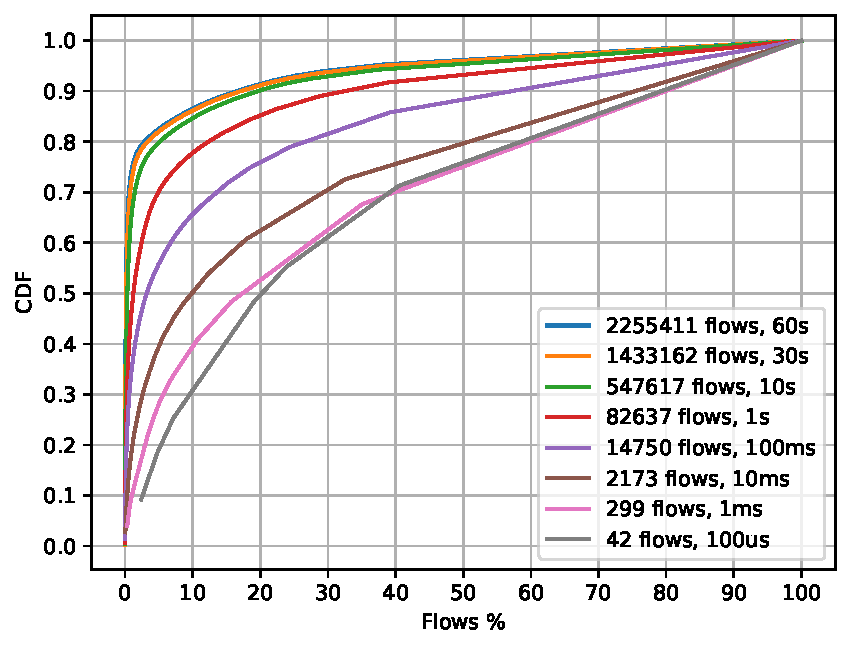
\includegraphics[width=0.26\textwidth]{fig_cdf_pkt.pdf}
			\label{fig:cdf_pkt}
		}%\qquad
		\subfloat[Size-weighted heavy hitter flows]{
			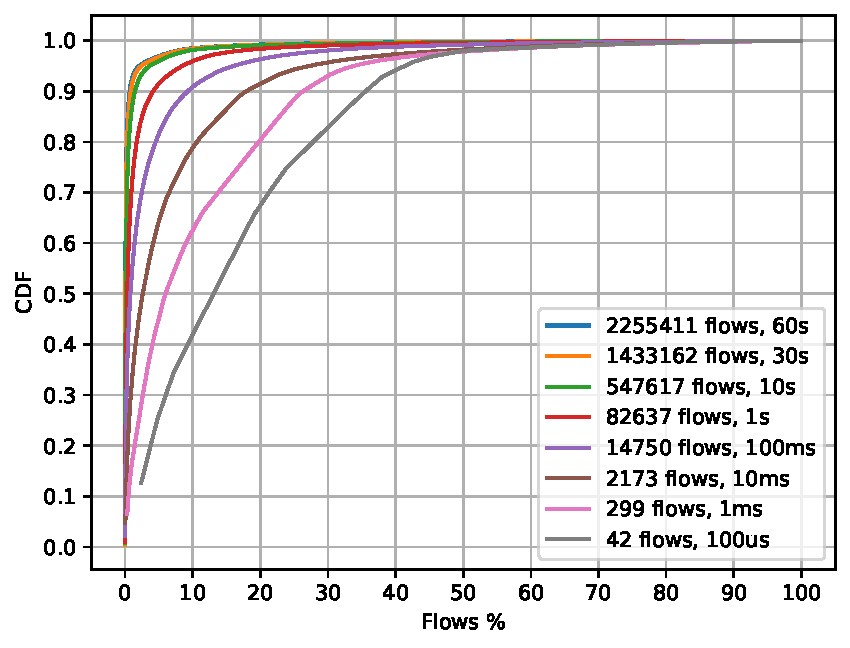
\includegraphics[width=0.26\textwidth]{fig_cdf.pdf}
			\label{fig:cdf}
		}%\\
		\subfloat[Flow duration]{
			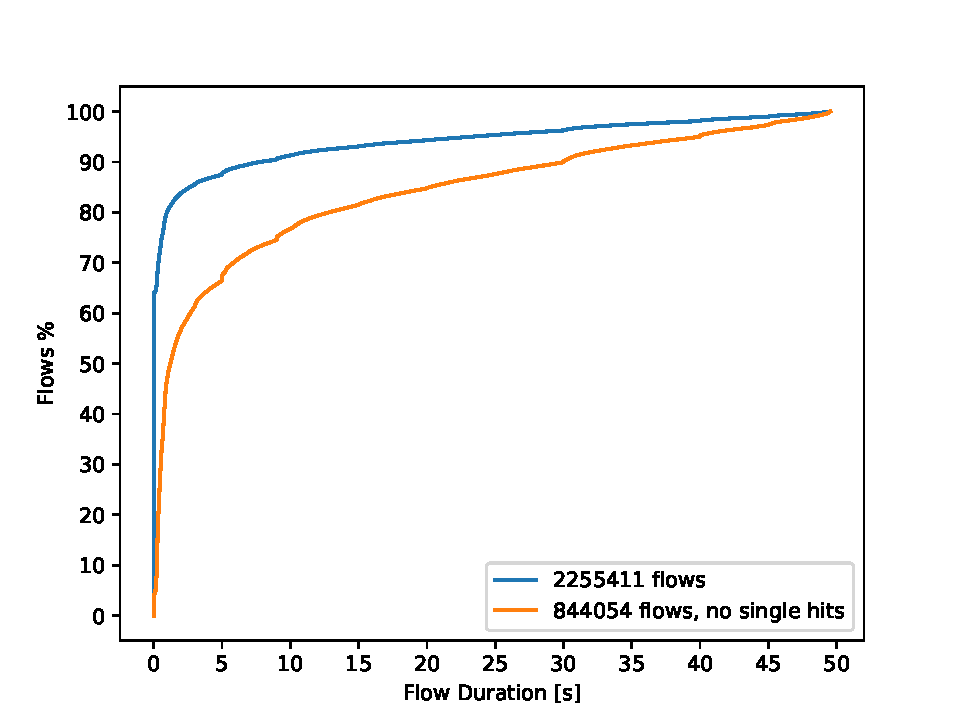
\includegraphics[width=0.26\textwidth]{fig_duration.pdf}
			\label{fig:flow_duration}
		}%\qquad
		\subfloat[Average flow size]{
			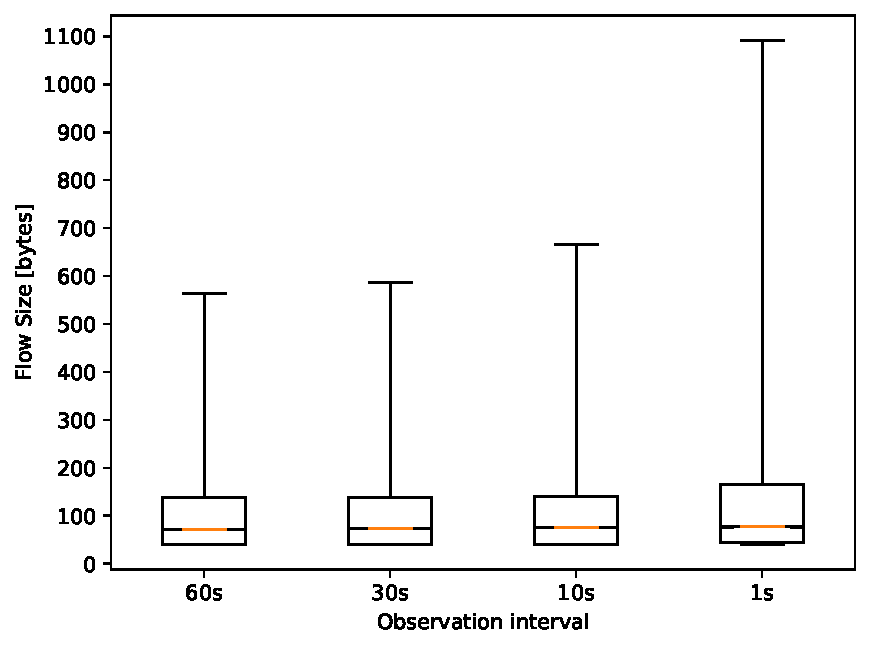
\includegraphics[width=0.26\textwidth]{fig_avg_flow_size.pdf}
			\label{fig:flow_size}
		}
		\caption{CAIDA trace summary}
		\label{fig:traces}
	\end{adjustwidth}
\end{figure*}


To that end, we borrow from the cache hierarchy concept of computer systems.
%In our system, a first-level cache is a high-performance but memory limited programmable ASIC.
%The FPGA plays the role of second-level cache, and finally the CPU is the last-level cache.
In our proposed caching system, a first-level cache is a high-performance but memory-limited PDD.
At every cache level, the performance metric $P_{k}$ (throughput in our case) is decreased, such that $P_{k} > P_{k+1}$.
Memory capacity is augmented to $M_{k}$, with $M_{k} < M_{k+1}$. 
The performance ratio between two successive cache levels is characterized by a processing slowdown factor $SF$ defined as $SF_{k} = \frac{P_{k-1}}{P_{k}}$.


However, match-action caching is fairly different from CPU caches.
First, temporal and spatial data locality is less predictable in network systems.
Second, memory is scarce and the processing flexibility is limited in network switches, thus, complex cache policies may not be suitable.
Third, due to dynamic traffic changes, a cache system needs to rapidly adapt to diversified workloads.
As a consequence, traditional caching schemes may not be suitable in the context of heterogeneous match table caching systems. 

%Thus, we propose a match-action cache policer split into the forwarding devices.
%We use online traffic hitters to estimate which match-action entries are candidates to be promoted/evicted to/from another cache level.
%We are inspired in previous works on flow caching \cite{casado:2008,Katta:2014,Pfaff:15} and on heuristic dataplane-based traffic hitters \cite{Sivaraman:17} aiming to maintain line-rate throughput and required cache update rate while minimizing the usage of scarce memory resources available in each device and reducing processing latency.

To properly characterize the aforementioned issues, we evaluated the feasibility of such an HDP caching system by characterizing an recent data center network traffic to understand its temporal locality.
Following the traffic analysis, we conducted cache simulations to evaluate and compare realistic cache policies to be implemented in HDPs.
Finally, we evaluated which cache policies are tailored for current programmable dataplanes.% and how they can be described in P4.

To the best of our knowledge, this work is the first to consider match-action table management for HDPs.
The contributions of this work are as follows: 

\begin{itemize}[noitemsep,topsep=0pt]
	\item an open-source match-action cache policer for HDPs;
	\item a real-world network traffic analysis to derive match-action caching premises~(\S\ref{sec:traffic});
	\item an evaluation of cache policies in the context of programmable dataplanes~(\S\ref{sec:policies}); and
	\item a model to estimate the performance and a feasibility study of a match-action caching system in an HDP~(\S\ref{sec:cache_results}).
\end{itemize}



%\begin{figure*}[t!]
%	\centering
%	\subfloat[Heavy hitter analysis]{
%		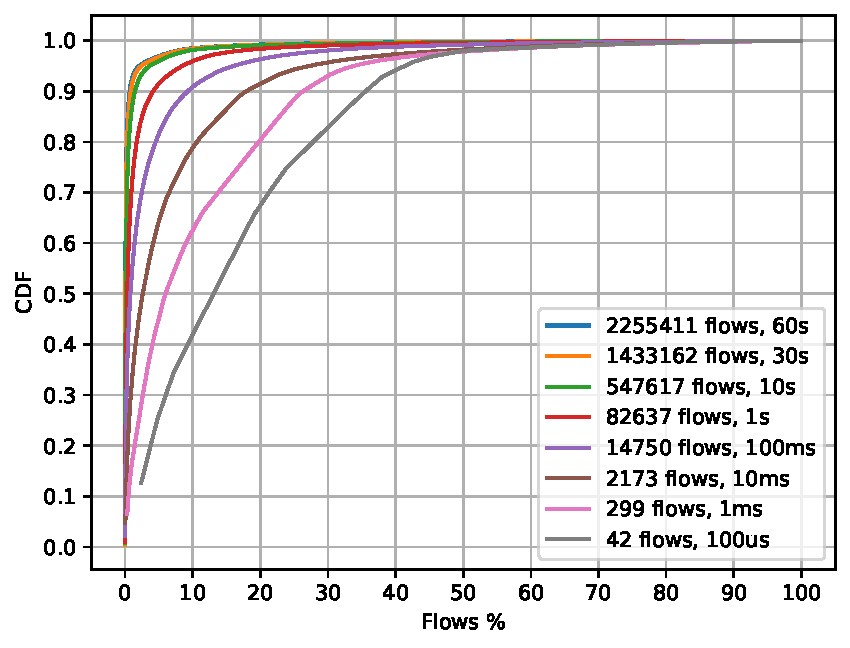
\includegraphics[width=0.33\textwidth]{fig_cdf.pdf}
%		\label{fig:cdf}
%	}
%	\subfloat[Flow duration]{
%		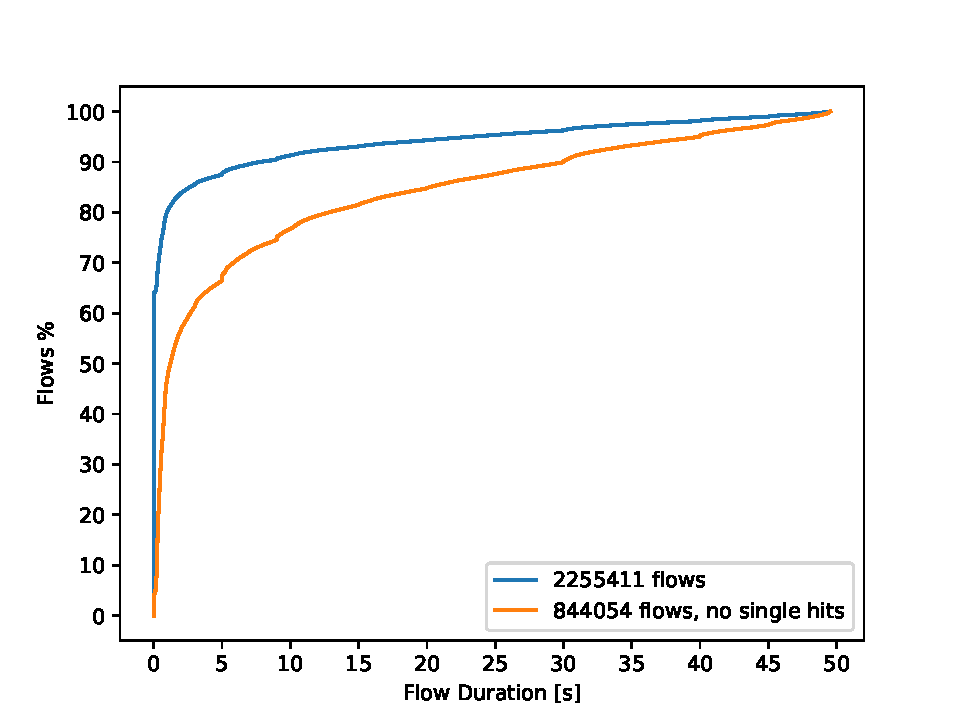
\includegraphics[width=0.33\textwidth]{fig_duration.pdf}
%		\label{fig:flow_duration}
%	}
%	\subfloat[Average flow size]{
%		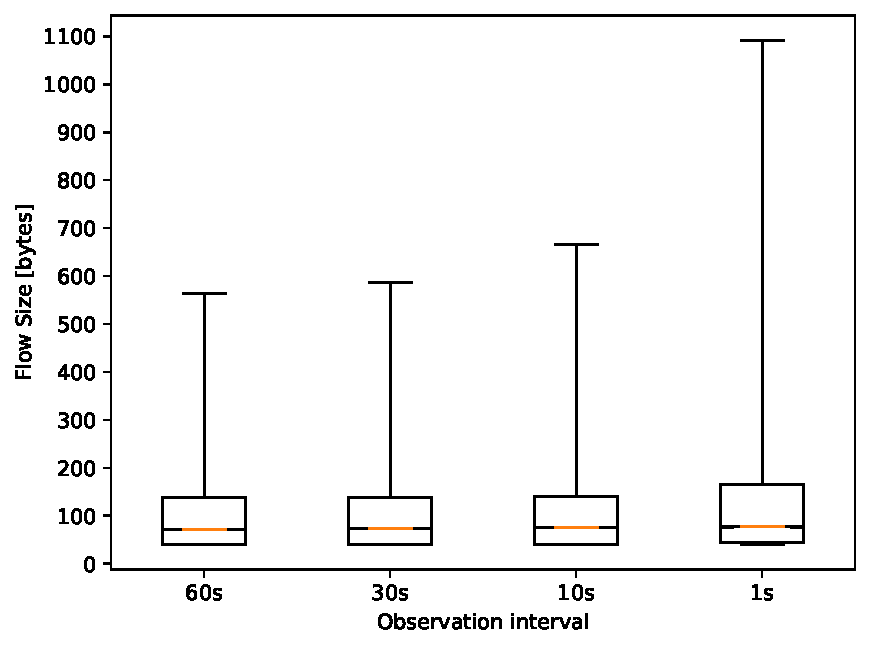
\includegraphics[width=0.33\textwidth]{fig_avg_flow_size.pdf}
%		\label{fig:flow_size}
%	}
%	\caption{CAIDA trace summary}
%	\label{fig:traces}
%\end{figure*}

\section{Learning from the Traffic}\label{sec:traffic}

Network traffic has been observed to follow a Zipf distribution as a few network flows account for most of the whole network traffic~\cite{Sarrar:2012,Jin:2017}.

In our study, we conducted experiments to determine the traffic characteristics of an up-to-date real-world data center trace.
We replayed a CAIDA network trace extracted from an IXP in a data center in New York dated from January 2019~\cite{caida:19}.
The analysed trace is 1 minute long monitoring $\sim$\SI{30}{\mega\nothing} packets in a full-duplex \SI{40}{\giga\bit/\second} Ethernet link connecting New York and S\~ao Paulo/Brazil.
A similar analysis was done by~\citeauthor{Spang:19} to estimate the number of TCP/IP flows~\cite{Spang:19}.

Figure~\ref{fig:traces} summarizes our observations.
In our analysis, we defined a flow as being a unique five-tuple $\langle$~IPv4/IPv6 Source IP address, IPv4/IPv6 destination IP address, L4 protocol, UDP/TCP source port, UDP/TCP destination port~$\rangle$ connection.

\textbf{Heavy hitters}~---~As shown in Figure~\ref{fig:cdf}, the Zipf distribution characteristic is still present in current network traffic.
The figure presents the CDF, in terms of transmitted bytes, for several observation intervals, ranging from \SI{100}{\micro\second} to \SI{60}{\second}.
For all observation intervals longer than \SI{100}{\milli\second}, fewer than 10\% of the flows dominate more than 90\% of the traffic.
For shorter intervals, the Zipf dominance is still present although more skewed.

\textbf{Flow duration}~---~Figure~\ref{fig:flow_duration} presents the flow duration time.
The blue curve is dominated (60\%) by single packet flows.
Single packet flows are represented with a flow duration of zero seconds.
Short-lived flows dominate the trace with $\sim$90\% of all flows lasting less than 5 seconds.
The orange curve in Figure~\ref{fig:flow_duration} illustrates the duration of flows with multiple hits in the trace.
Still, short-lived flows dominate the trace with $\sim$50\% lasting less than 1 second in the trace.

\textbf{Flow size}~---~Figure~\ref{fig:flow_size} presents the average flow size for four statistically representative observation intervals.
For all four measures, the first quartile, the median, and the third quartile are very similar.
On average, small flows ($\sim$100 bytes) dominate the trace with 75\% of the flows being no larger than 150 bytes.

According to our experiments, the expected Zipf distribution characteristic of network traffic is still present in current data center traffic.
Such characteristic favors flow caching in memory scarce programmable dataplanes.
However, we notice that short-lived flows dominate the trace.
Therefore, the chosen cache policy algorithm needs a fast reaction time to quickly adapt to traffic changes.
Besides, such temporal traffic characteristic possibly favors time-aware cache policies (e.g. LRU).

\section{Cache Replacement Algorithms}\label{sec:policies}

\subsection{Cache Eviction Policies}

\textbf{OPT}~---~The optimal (OPT) replacement policy~\cite{Belady:66} is an oracle algorithm that relies on knowing the future traffic behavior.
OPT uses this information to replace data that is further referenced in time.
Due to that, OPT is not realistically implementable and it is commonly used to evaluate cache performance since it sets an upper performance bound for realistic caching systems.

\textbf{Random}~---~Random or pseudo-random replacement policies use a stochastic random function to select a victim for eviction.
Pseudo-random cache policy has been widely adopted in ARM-based processors.
In random policies, no history on cache misses/hits nor cache access frequency is required.
The efficiency of a random policy is directly related to the quality of its random generator function.

\textbf{LRU}~---~The LRU replacement algorithm evicts the most ancient cache entry in case of a cache miss.
A possible LRU implementation uses a timestamp tag to sort cache entries by recency, as in Algorithm~\ref{algo:lru}.

\begin{algorithm}[]
	\caption{LRU policy}
	\label{algo:lru}
	\SetInd{0.1em}{.9em}
	\SetAlgoLined
	\footnotesize
	\SetKwProg{procedure}{Procedure}{}{end}
	\SetKwFunction{minTimestampEntry}{minTimestampEntry}
	\SetKwFunction{findEntry}{findEntry}
	\SetKwFunction{lruPolicy}{lruPolicy}
	\SetKwInOut{Input}{input}
	\SetKw{In}{in}%
	\SetKw{Not}{not}%
	\SetKw{Or}{or}%
	\SetKw{Continue}{continue}%
	\SetKw{True}{true}%
	\Input{Cache memory: list of $\langle$\texttt{entry, timestamp}$\rangle$ pairs}
	\Input{Possible cache entry}
	\Input{Packet timestamp}
	\procedure{\lruPolicy{cache, possible\_entry, current\_timestamp}}{
		\If(\hfill\tcp*[h]{Cache hit}){possible\_entry \In cache}{
			entry\_found =  \findEntry{cache, possible\_entry}\hfill\tcp{Hit pointer}
			entry\_found$\rightarrow$timestamp  = current\_timestamp
		}
		\Else(\hfill\tcp*[h]{Cache Miss}){
			victim = \minTimestampEntry{cache}\hfill\tcp{Victim pointer}			
			*victim = $\langle$possible\_entry, current\_timestamp$\rangle$
		}
	}
\end{algorithm}

\textbf{LFU}~---~Contrarily to LRU, LFU uses hit frequency rather than the access time to evict entries.
LFU uses a frequency counter to sort cache entries by frequency.
In case of a hit, the frequency counter is incremented.
Otherwise, the cache entry with the lowest frequency is chosen for eviction, as in Algorithm~\ref{algo:lfu}.

\begin{algorithm}[]
	\caption{LFU policy}
	\label{algo:lfu}
	\SetInd{0.1em}{.9em}
	\SetAlgoLined
	\footnotesize
	\SetKwProg{procedure}{Procedure}{}{end}
	\SetKwFunction{lfuPolicy}{lfuPolicy}
	\SetKwFunction{findEntry}{findEntry}
	\SetKwFunction{minFrequencyEntry}{minFrequencyEntry}
	\SetKwInOut{Input}{input}
	\SetKw{In}{in}%
	\SetKw{Not}{not}%
	\SetKw{Or}{or}%
	\SetKw{Continue}{continue}%
	\SetKw{True}{true}%
	\Input{Cache memory: list of $\langle$\texttt{entry, counter}$\rangle$ pairs}
	\Input{Possible cache entry}
	\procedure{\lfuPolicy{cache, possible\_entry}}{
		\If(\hfill\tcp*[h]{Cache hit}){possible\_entry \In cache}{
			entry\_found = \findEntry{cache, possible\_entry}\hfill\tcp{Hit pointer}
			entry\_found$\rightarrow$counter  += 1
		}
		\Else(\hfill\tcp*[h]{Cache miss}){
			victim =  \minFrequencyEntry{cache}\hfill\tcp{Victim pointer}
			*victim = $\langle$possible\_entry, 1$\rangle$
		}
	}
\end{algorithm}

\textbf{WLFU}~---~\textit{Vanilla} implementations of LFU perform poorly with real-world network traces~\cite{Kim:09}.
\textit{Vanilla} LFU considers all cache hits with equal weight, which is not realistic in network communications because larger packets incur in greater network efficiency compared to small ones.
Thus, Weighted LFU (WLFU) leverages \textit{vanilla} LFU by considering the packet size in its frequency counters.
A possible implementation of WLFU is illustrated in Algorithm~\ref{algo:wlfu}.

\begin{algorithm}[]
\caption{WLFU policy}
\label{algo:wlfu}
\SetInd{0.1em}{.9em}
\SetAlgoLined
\footnotesize
\SetKwProg{procedure}{Procedure}{}{end}
\SetKwFunction{wlfuPolicy}{wlfuPolicy}
\SetKwFunction{findEntry}{findEntry}
\SetKwFunction{minFrequencyEntry}{minFrequencyEntry}
\SetKwInOut{Input}{input}
\SetKw{In}{in}%
\SetKw{Not}{not}%
\SetKw{Or}{or}%
\SetKw{Continue}{continue}%
\SetKw{True}{true}%
\Input{Cache memory: list of $\langle$\texttt{entry, counter}$\rangle$ pairs}
\Input{Possible cache entry}
\Input{Packet Size}
\procedure{\wlfuPolicy{cache, possible\_entry, pkt\_size}}{
	\If(\hfill\tcp*[h]{Cache hit}){possible\_entry \In cache}{
		entry\_found =  \findEntry{cache, possible\_entry}\hfill\tcp{Hit pointer}
		entry\_found$\rightarrow$counter  += pkt\_size\hfill\tcp{Increment size counter}
	}
	\Else(\tcp*[h]{Cache miss}){
		victim =  \minFrequencyEntry{cache}\hfill\tcp{Victim pointer}
		*victim = $\langle$possible\_entry, pkt\_size$\rangle$
	}
}
\end{algorithm}

\textbf{OLFU}~---~Optmistic LFU (OLFU) is a proposition to overcome the limitations of \textit{vanilla} LFU for flow caching.
OLFU is an LFU derivation that gives a chance for a cache promotion candidate to remain in cache regardless of its \textit{actual} hit frequency.
In OLFU, the cache policer behaves as the \textit{vanilla} LFU in case of a cache hit.
Otherwise, instead of re-initializing the frequency counter, the new cache entry takes control of the victim's counter, as shown in Algorithm~\ref{algo:olfu}.

\begin{algorithm}[]
\caption{OLFU policy}
\label{algo:olfu}
\SetInd{0.1em}{.9em}
\SetAlgoLined
\footnotesize
\SetKwProg{procedure}{Procedure}{}{end}
\SetKwFunction{olfuPolicy}{olfuPolicy}
\SetKwFunction{findEntry}{findEntry}
\SetKwFunction{minFrequencyEntry}{minFrequencyEntry}
\SetKwInOut{Input}{input}
\SetKw{In}{in}%
\SetKw{Not}{not}%
\SetKw{Or}{or}%
\SetKw{Continue}{continue}%
\SetKw{True}{true}%
\Input{Cache memory: list of $\langle$\texttt{entry, counter}$\rangle$ pairs}
\Input{Possible cache entry}
\procedure{\olfuPolicy{cache, possible\_entry}}{
	\If(\hfill\tcp*[h]{Cache hit}){possible\_entry \In cache}{
		entry\_found =  \findEntry{cache, possible\_entry}\hfill\tcp{Hit pointer}
		entry\_found$\rightarrow$counter  += 1
	}
	\Else(\hfill\tcp*[h]{Cache miss}){
		victim = \minFrequencyEntry{cache}\hfill\tcp{Victim pointer}
		*victim = $\langle$possible\_entry, victim$\rightarrow$counter + 1$\rangle$\hfill\tcp{Replace reusing current counter}
	}
}
\end{algorithm}


\textbf{OWLFU}~---~To optimize cache efficiency, OWLFU combines the OLFU and WLFU cache policies.
In case of a hit, OWLFU behaves as WLFU.
Otherwise, OWLFU modifies OLFU by incrementing the current packet size to the victim frequency counter, as in Algorithm~\ref{algo:owlfu}.

\begin{algorithm}[]
\caption{OWLFU policy}
\label{algo:owlfu}
\SetInd{0.1em}{.9em}
\SetAlgoLined
\footnotesize
\SetKwProg{procedure}{Procedure}{}{end}
\SetKwFunction{owlfuPolicy}{owlfuPolicy}
\SetKwFunction{findEntry}{findEntry}
\SetKwFunction{minFrequencyEntry}{minFrequencyEntry}
\SetKwInOut{Input}{input}
\SetKw{In}{in}%
\SetKw{Not}{not}%
\SetKw{Or}{or}%
\SetKw{Continue}{continue}%
\SetKw{True}{true}%
\Input{Cache memory: list of $\langle$\texttt{entry, counter}$\rangle$ pairs}
\Input{Possible cache entry}
\Input{Packet Size}
\procedure{\owlfuPolicy{cache, possible\_entry, pkt\_size}}{
	\If(\hfill\tcp*[h]{Cache hit}){possible\_entry \In cache}{
		entry\_found =  \findEntry{cache, possible\_entry}\hfill\tcp{Hit pointer}
		entry\_found$\rightarrow$counter  += pkt\_size\hfill\tcp{Increment size counter}
	}
	\Else(\hfill\tcp*[h]{Cache miss}){
		victim =  \minFrequencyEntry{cache}\hfill\tcp{Victim pointer}
		*victim = $\langle$possible\_entry, victim$\rightarrow$counter + pkt\_size$\rangle$\hfill\tcp{Replace reusing current size counter}
	}
}
\end{algorithm}

\subsection{Cache Promotion Policies}
Describe here why the need of a cache promotion policy and which ones we studied.

\section{Evaluating Cache Perfomance}\label{sec:cache_results}

\begin{figure*}[]
\centering
\subfloat[Hit Ratio. $SF=1\times$]{
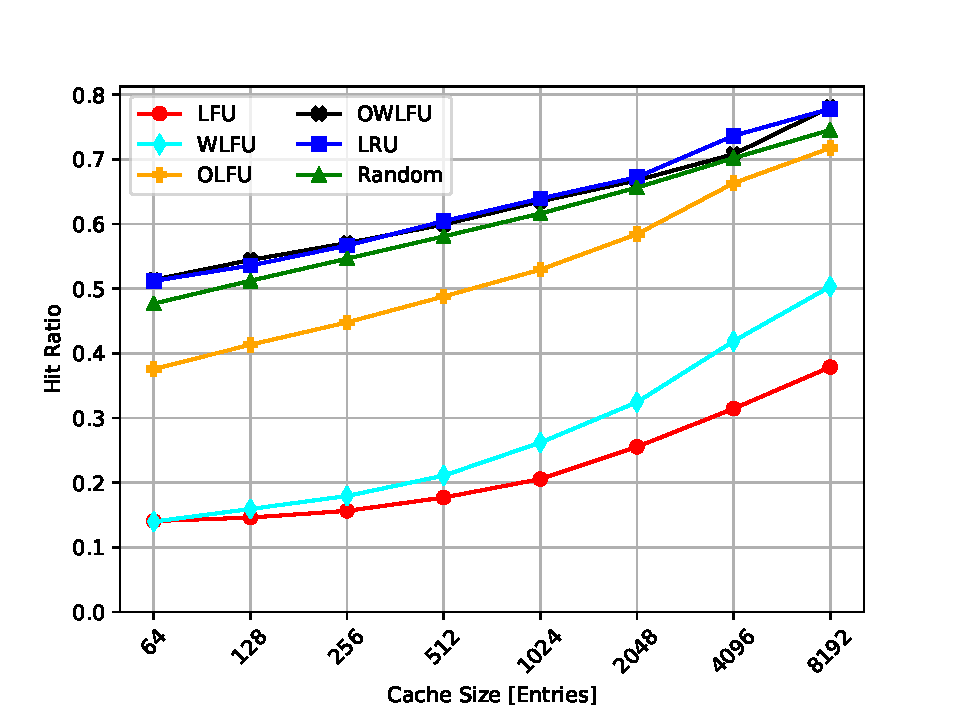
\includegraphics[width=0.33\textwidth]{hit_ratio_sf1.pdf}
\label{fig:hit_ratio_sf1}
}
\subfloat[Hit Ratio. $SF=10\times$]{
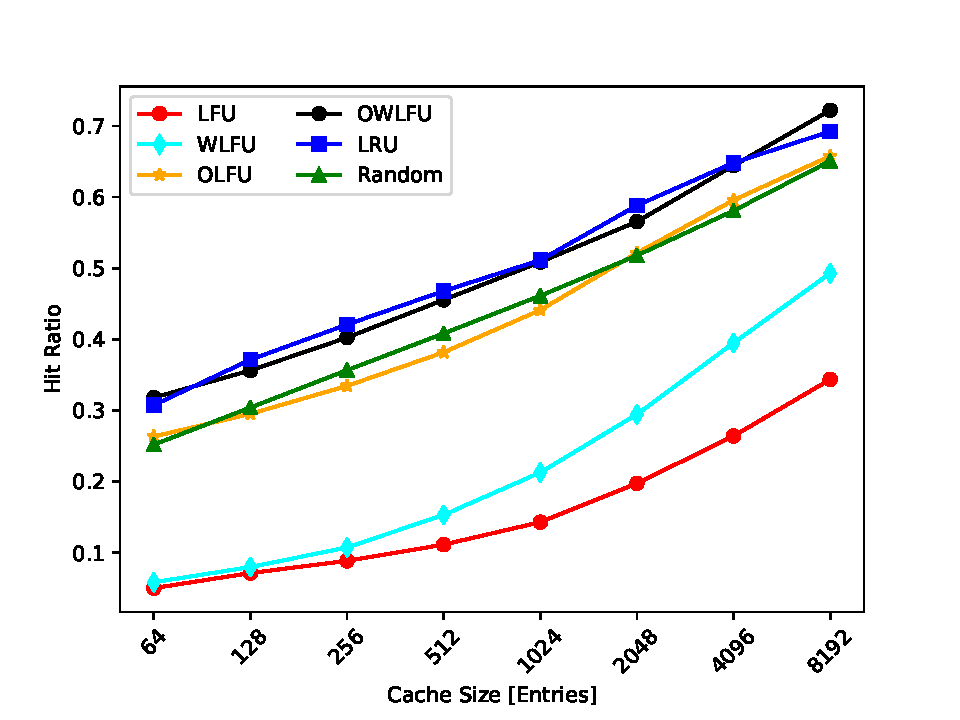
\includegraphics[width=0.33\textwidth]{hit_ratio_sf10.pdf}
\label{fig:hit_ratio_sf10}
}
\subfloat[Hit Ratio. $SF=100\times$]{
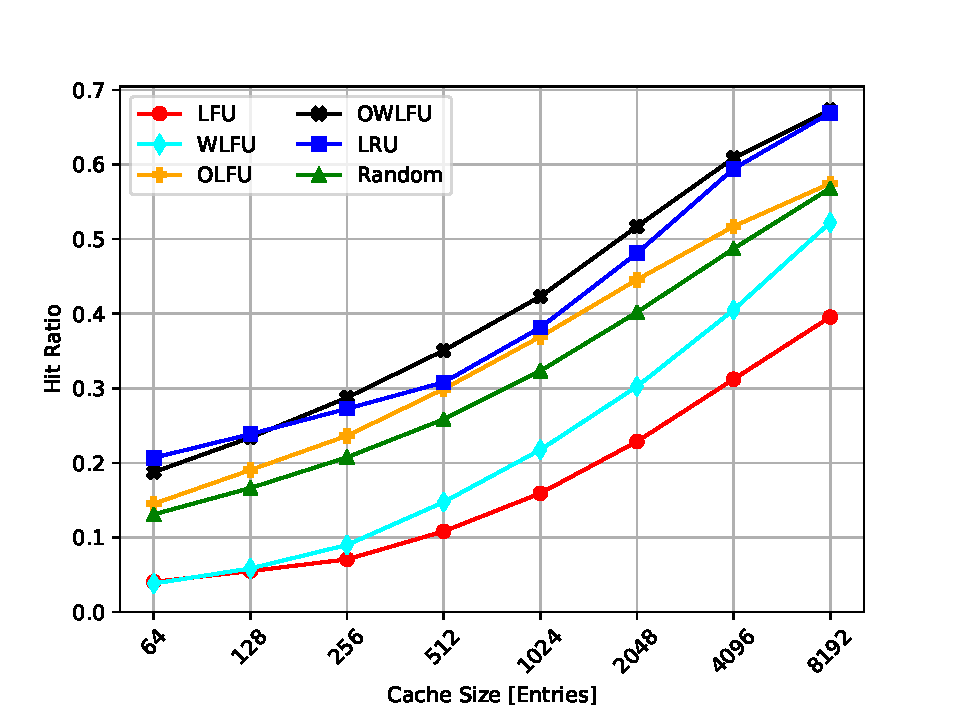
\includegraphics[width=0.33\textwidth]{hit_ratio_sf100.pdf}
\label{fig:hit_ratio_sf100}
}\\
\subfloat[Size Weighted Hit Ratio. $SF=1\times$]{
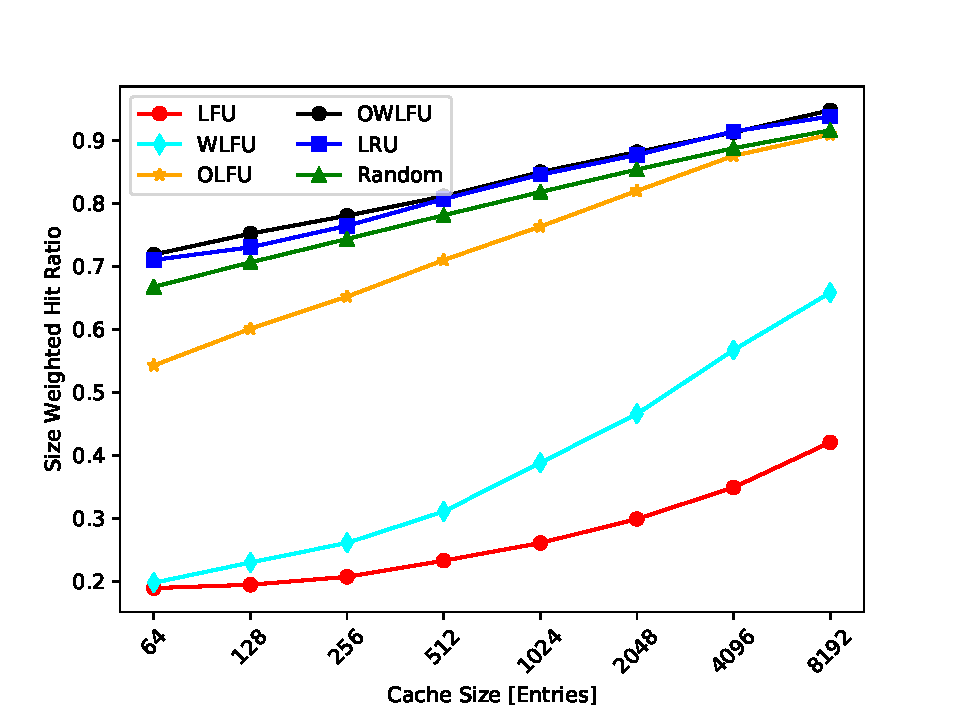
\includegraphics[width=0.33\textwidth]{weighted_hit_ratio_sf1.pdf}
\label{fig:weighted_hit_ratio_sf1}
}
\subfloat[Size Weighted Hit Ratio. $SF=10\times$]{
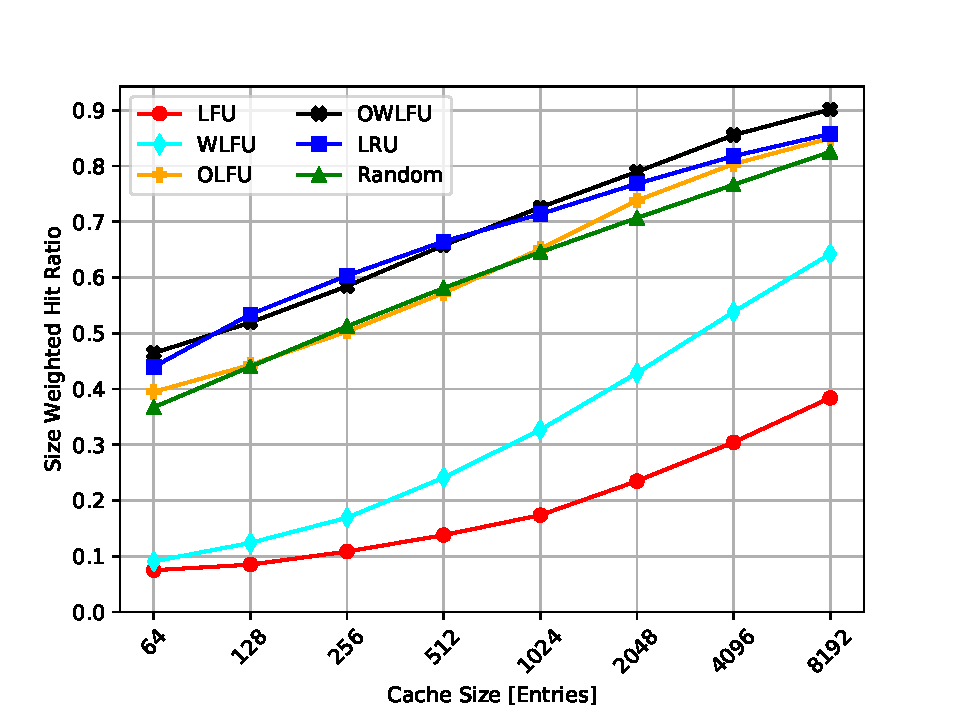
\includegraphics[width=0.33\textwidth]{weighted_hit_ratio_sf10.pdf}
\label{fig:weighted_hit_ratio_sf10}
}
\subfloat[Size Weighted Hit Ratio. $SF=100\times$]{
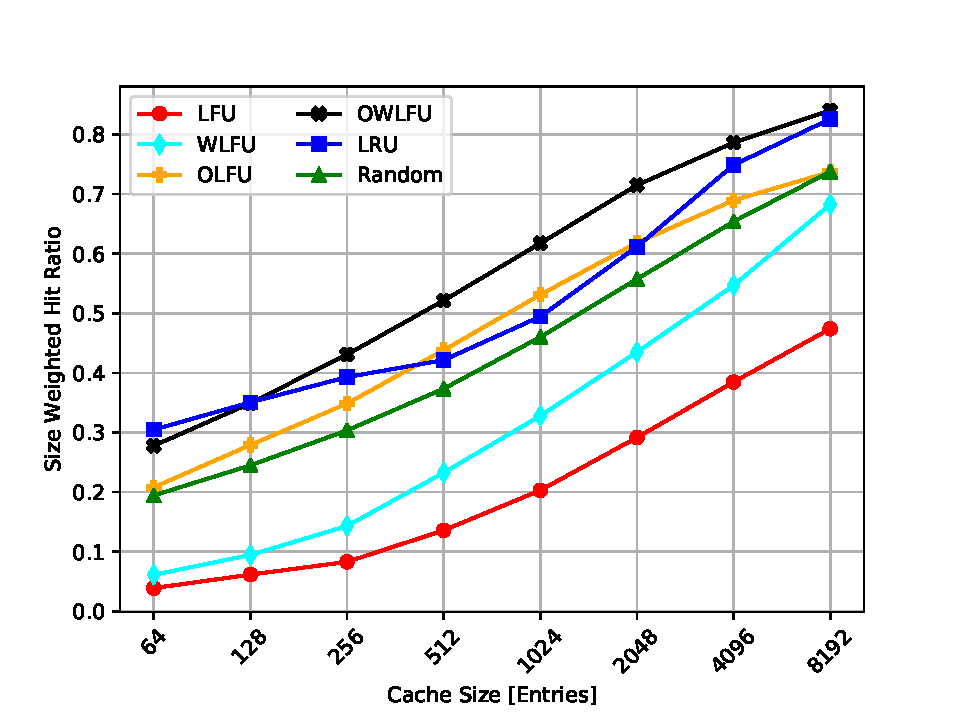
\includegraphics[width=0.33\textwidth]{weighted_hit_ratio_sf100.pdf}
\label{fig:weighted_hit_ratio_sf100}
}
\caption{Cache performance evaluation}
\label{fig:hit_ratio}
\end{figure*}


\subsection{Experimental Setup}
Table~\ref{tab:setup} presents the simulation parameters used to evaluate a two-level caching system as in Figure~\ref{fig:high_level_network}
We simulated the cache performance by emulating different cache policer slowdown factor ($SF$).
Note, that for a two-level caching scheme, $SF$ also represents the cache policer reaction time.
As performance metrics, we reported the cache hit ratio and the traffic size weighted hit ratio.
%The term slowdown factor ($SF$) refers to the cache policer reaction time.
%The slowdown factor is relative to the cache speed, i.e., a slowdown of 10$\times$ means that the cache policer is 10$\times$ slower than a cache access.
%The presented results were generated using the IXP New York to S\~ao Paulo data center trace~\cite{caida:19}.
The simulated traffic trace is the same as in~\S\ref{sec:traffic}.
To enable reproducibility, we open-sourced our codes\footnote{\url{https://github.com/engjefersonsantiago/Infinite_MT}.}.


\begin{table}[h]
	\centering
	\caption{Experimental Parameters}
	\label{tab:setup}
	\begin{tabular}{|l|l|}
		\hline
		\textbf{Parameter}       & \textbf{Value}   \\
		\hline
		Cache policy            & LRU, (O)(W)LFU, Random			    \\
		Cache Size              & 64 to \SI{8}{\kilo\nothing} entries  \\
		Slowdown Factor         & 1$\times$, 10$\times$, 100$\times$        \\
		\hline
	\end{tabular}
\end{table}

\subsection{Results}
Figure~\ref{fig:hit_ratio} presents the results for our experiments when no promotion policy is implemented.

As already reported in~\cite{Kim:09}, \textit{vanilla} LFU performs poorly with real-world network traffic.
Also, we confirmed the good performance of LRU-based policies with up-to-date data center traffic. 
The random policy achieves a relative good cache performance considering the small overhead for implementing it.
Random policy hit ratio lags behind the classic LRU by no more than 10 percentage points.

All modified versions of LFU significantly improve the cache performance compared to the \textit{vanilla} LFU.
WLFU observes a sharp increase in its hit ratio as the cache size increases.
OLFU observes a steady performance approaching the random hit ratio.
Indeed, OLFU introduces a pseudo-temporal variable to the LFU policy because it speculates that the promoted cache entry will be referenced in a near future. 
Last, OWLFU performs best in almost all scenarios.
This is nonetheless expected since it combines the strengths of OLFU and WLFU.

TODO: Check and run OPT simulations.

TODO: Comment the SF effect.

TODO: Evaluate the promotion policy.
\section{Related Work}\label{sec:related_works}

Flow caching has been studied since the early times in flow-based networking.
\citeauthor{casado:2008}~\cite{casado:2008} remarked in 2008 that a hardware-based SDN switch must achieve over 99\% hit-ratio to avoid system bottlenecks due to software interaction.

Since then, flow caching has been explored for both hardware and software solutions.
\citeauthor{Kim:09}~\cite{Kim:09} revisited cache policies in the context of IP networks.
\citeauthor{Katta:2014}~\cite{Katta:2014,Katta:2016} addressed the issue of limited TCAM resources in hardware switches by proposing a hybrid hardware-software switch to exploit memory-abundant CPUs.
The cache policy algorithm, however, is performed offline. 
From the software side, the Open vSwitch (OVS) has employed flow caching since its inception \cite{Pfaff:15}.
In OVS, the flow cache is split into two levels, microflow and megaflow.
The microflow caches at a fine granularity for long-lasting connections while the megaflow, at coarser granularity, takes care of short-lived flows.

\citeauthor{Grigoryan:18} proposed a programmable FIB caching architecture~\cite{Grigoryan:18}.
They were inspired by the heavy-hitter implementation of \citeauthor{Sivaraman:17}~\cite{Sivaraman:17} to detect and evict infrequent TCAM entries.
However, their approach requires data-plane based learning for cache replacement and it assumes that the switch can deal with variable lookup time, which compromises performance due to pipeline stalls. 

\citeauthor{Zhang:2018} presented B-cache, a behavior-level cache for programmable dataplanes~\cite{Zhang:2018}. Similarly to \citeauthor{Grigoryan:18}~\cite{Grigoryan:18}, the authors exploit heavy-hitters to identify hot behavior in programmable dataplanes, which in turn could be cached. Similarly, this work is infeasible in current homogeneous high-performance switches since it breaks the streaming flow throughout the pipeline.

\citeauthor{Kim:2018} proposed extending the memory capacity in programmable switches by borrowing memory resources from RDMA-capable servers in data centers~\cite{Kim:2018}. However, the achieved latency can be in the order of microseconds and the switch does not consider any cache policy mechanism.

%\textit{Traffic Hitters} have mainly been used for network monitoring and management with the goal of identifying hot network behavior, and potential attacks. Realistic implementations of traffic hitters have mainly used sketch algorithms and their variations \cite{Cormode:05,Cormode:08,Metwally:05} in order to increase memory efficiency. Liu \textit{et al. } \cite{Liu:16} have deployed network-wide flow monitoring. Sivaraman \textit{et al. } \cite{Sivaraman:17} have adapted the classical finding the top-k element problem \cite{Metwally:05} to map it efficiently to programmable switches \cite{Bosshart:13}. FPGA-based deployments have also been proposed \cite{Tong:13,Tong:16,Zazo:17}.

\section{Conclusion}\label{sec:conclusion}

P4 and the PISA architecture are bringing a new meaning to programmable networks as they promote data plane programming.
Although current PISA-based programmable dataplanes offer high throughput, they lack memory resources for implementing P4 applications.
Thus, recent research proposed heterogeneous dataplanes to confront the memory/performance trade-off.
However, the problem heterogeneous match table caching has not yet been addressed.

In this work, we presented a cache hierarchy for HDPs.
We analyzed real-world data center network traces to derive caching premises.
Based on our observations, we proposed new traffic-aware cache eviction and promotion policies.
These new policies, alongside classic ones, were evaluated in the context of HDPs.
Simulation results show a size weighted hit ratio approaching 90\% when HDP-realistic cache policies (Random+WMFU) are used.
Moreover, the theoretical OWLFU eviction policy outperforms other policies when no promotion policy is implemented.
This may motivate future research on approximating OWLFU targeting data plane realization.

%\section{Introduction}\label{sec:intro}

The Software-Defined Networking (SDN) paradigm has brought programmability to the once rigid network ecosystem. By allowing both control and data planes to evolve independently, SDN has opened new research avenues in networking, including data plane programming. Notably, the P4 language is a result of the SDN convergence \cite{Bosshart:14}. P4 leverages OpenFlow by allowing network administrators to program their network in a custom fashion. Thanks to P4 and recent programmable dataplanes \cite{Bosshart:13}, they can now deploy custom protocols by reprogramming network switches according to evolving needs, without deploying expensive new hardware. 


However, current data center networks (DCNs) requirements are such \textcolor{red}{[ref]} that even state-of-the-art programmable ASICs \cite{tofino:18} cannot solely meet them. Next generation mobile communication (5G) requirements, for instance, include multi-million active sessions ($>$\SI{5}{\mega\nothing}) at terabit rates and stringently low end-to-end latency ($<$\SI{1}{\milli\second}), possibly running over custom protocols.

Recently, some research has suggested using heterogeneous programmable data planes (HDPs) to alleviate data center network switch bottlenecks \cite{p4eu:18}. Indeed, using complementary and distinct packet forwarding devices increases the overall switch processing capabilities. However, research regarding HDPs is still in its infancy with many questions to be solved, including the development of heterogeneous compilers, mismatched processing capabilities and hardware resources, and match-tables management.

In this work, we address the issue of match-action (M-A) table management in HDPs comprising a high speed programmable ASIC, an FPGA, and a host CPU. To that end, we borrow the cache hierarchy concept of regular computer systems. In our system, a first-level cache is the high-performance but memory limited programmable ASIC. The FPGA plays the role of second-level cache, and finally the CPU is the last-level cache. M-A caching is fairly different from regular CPU cache systems since temporal and spatial data locality are difficult to predict in network systems. 

Thus, we propose a M-A cache policer split into the forwarding devices. We use online traffic hitters to estimate which M-A entries are candidates to be promoted/evicted to/from another cache level. We are inspired in previous works on flow caching \cite{casado:2008,Katta:2014,Pfaff:15} and on heuristic dataplane-based traffic hitters \cite{Sivaraman:17} aiming to maintain line-rate throughput and required cache update rate while minimizing the usage of scarce memory resources available in each device and reducing processing latency.

To the best of our knowledge, our work is the first to consider a M-A cache policer for HDPs. The contributions of this work are as follows: 
\begin{itemize}[noitemsep,topsep=0pt]
	\item an open-source P4-based match-action cache policer for HDPs (\S\ref{sec:method});
	\item a model to estimate the performance and overhead of a M-A cache system in an HDP (\S\ref{sec:model}); and
	%\item a P4-based emulation prototyping platform (\S\ref{sec:emulation}). 
	\item a P4-based emulation platform for rapid performance estimation (\S\ref{sec:emulation}); and 
	\item a prototype comprising a programmable ASIC, an FPGA, and a CPU.
\end{itemize}

%The rest of this paper is organized as follows. Section~\ref{sec:eco_pro} presents the ecosystem this work is inserted into and states the problem that we propose to solve. Section~\ref{sec:related_works} reviews the literature, Section~\ref{sec:method} presents the proposed match-action cache policer, Section~\ref{sec:results} shows the experimental results and discussions, and Section~\ref{sec:conclusion} draws the conclusions.


\section{Network Ecosystem and Problem Statement}\label{sec:eco_pro}

%In this section, we first introduce the ecosystem in which our work is inserted into by presenting terms and definitions used in this paper. Then, we state the problem that this work proposes to solve.

In this section, we first introduce the ecosystem in which our work is inserted into, and then, we state the problem that this work proposes to solve.

\subsection{Network Ecosystem}\label{sec:eco}

In this paper, we consider an SDN switch for a leaf-spine data center network as illustrated in Figure~\ref{fig:high_level_network}. In the figure, solid lines indicate the data plane and dashed lines refer to control plane communication. Dotted lines delimit the cache levels of an HDP. The next paragraphs describe terms and definitions used throughout this text.

\begin{figure}[]
	\centering
	%\begin{tikzpicture}[node distance = 0.5cm, every node/.style={draw}, node font={\footnotesize}]
%%software
%\begin{scope}[every node/.style={draw, chamfered rectangle, chamfered rectangle corners=north east}]
%	\node (globp4) {P4};
%	\node[rectangle, right=of globp4] (compiler) {HDP compiler};
%	\node[below= 0.5cm of compiler] (p4cpu2) { P4};
%	\node[left= of p4cpu2] (p4cpu1) {P4};
%	\node[left= of p4cpu1] (p4fpga1) {P4};
%	\node[right= of p4cpu2] (p4fpga2) {P4};
%	\node[right= of p4fpga2] (p4asic) { P4};
%%%path for the corner of p4 codes
%	\path[draw]  (globp4.before north east) -| (globp4.after north east)
%							  (p4cpu2.before north east) -| (p4cpu2.after north east)
%							  (p4cpu1.before north east) -| (p4cpu1.after north east)
%						      (p4fpga1.before north east) -| (p4fpga1.after north east)
%							  (p4fpga2.before north east) -| (p4fpga2.after north east)
%							  (p4asic.before north east) -| (p4asic.after north east);
%
%%%compilation
%	\begin{scope}[every node/.style={rectangle, draw, align=center}, node distance=0.25cm]
%		\node[below= of p4cpu2] (compcpu2) { CPU\\ comp};
%		\node[below= of p4cpu1] (compcpu1) { CPU\\ comp};
%		\node[below= of p4fpga1] (compfpga1) { FPGA\\ comp};
%		\node[below= of p4fpga2] (compfpga2) { FPGA\\ comp};
%		\node[below= of p4asic] (compasic) { ASIC\\ comp};
%	\end{scope}
%%%processus
%	\begin{scope}[every edge/.style={-Stealth, draw}]
%   \coordinate (midBelowComp) at ($(compiler.south) - (0,0.25)$);
%	\path[draw] (globp4) edge (compiler)
%	    							  (compiler.south) edge (p4cpu2)
%								  ($(compiler.south) - (0.2,0)$) |- ( p4cpu1.north |- midBelowComp) edge (p4cpu1)
%                                  ($(compiler.south) - (0.4,0)$) |- ($( p4fpga1.north |- midBelowComp) + (0,0.1)$) edge (p4fpga1)
%								 ($(compiler.south) + (0.2,0)$) |- ( p4fpga2.north |- midBelowComp) edge (p4fpga2)
%                                  ($(compiler.south) + (0.4,0)$) |- ($( p4asic.north |- midBelowComp) + (0,0.1)$) edge (p4asic)
%								 (p4cpu1) edge (compcpu1)
%								 (p4cpu2) edge (compcpu2)
%								 (p4fpga1) edge (compfpga1)
%								 (p4fpga2) edge (compfpga2)
%								 (p4asic) edge (compasic)
%									;
%	\end{scope}
%
%\end{scope}
%\coordinate (midCPU) at ($(p4cpu1.east |- compcpu1.south) + (0.25cm, -0.5cm)$);
%%%hardware
%\begin{scope}[every node/.style={draw},]
%	\node[left=0.25cm of midCPU, anchor=north east] (cpu1) {CPU\textsubscript{1}};
%	\node[right=0.25cm of midCPU, anchor=north west] (cpu2) {CPU\textsubscript{2}};
%	\node[below=of cpu1, fill=black!20] (fpga1) {FPGA\textsubscript{1}};
%	\node[below=of cpu2] (fpga2) {FPGA\textsubscript{2}};
%	\node[fill=black!20, minimum width=2.25cm, anchor = north] (asic) at ($(midCPU|-fpga2.south) - (0,0.5)$) {ASIC};
%	\node[draw=none,left =0.55 of asic, align=left] (data_label) {};
%	
%\end{scope}
%\node[fit=(cpu1) (cpu2) (fpga1) (fpga2) (asic) (data_label), rounded corners] (platform) {};
%\node[draw=none, anchor=west] at (platform.west |- asic.east) {HDP};
%\node[cloud, draw, aspect=2, inner sep=-2pt, below=0.4cm of asic] (network) {Network};
%\begin{scope}[every edge/.style={Stealth-Stealth, draw}]
%\path (cpu1) edge (cpu2)
%			(cpu1) edge (fpga1)
%			(cpu2) edge (fpga2)
%			(fpga1.south) edge (fpga1.south |- asic.north)
%			(fpga2.south) edge (fpga2.south |- asic.north)
%			;
%\end{scope}
%\begin{scope}[every edge/.style={thick, -Latex, dashed, draw}, every path/.style={thick, dashed}]
%		\path[draw] ($(platform.west |- compfpga1.south) - (0.1,0)$) -- ($(platform.west |- fpga1) - (0.1,0)$)  edge (fpga1)
%								(compfpga2) -- (compfpga2 |- fpga2) edge (fpga2)
%								(compasic) -- (compasic |- asic) edge (asic)
%								(compcpu2) edge (compcpu2.south |- cpu2.north) 
%								(compcpu1) edge (compcpu1.south |- cpu1.north) 
%								;
%	\end{scope}
%\path[Stealth-Stealth, draw] (network) edge (asic.south)
% 							   (network) edge ($(asic.south) + (0.2,0cm)$)
% 							   (network) edge ($(asic.south) - (0.2,0cm)$)
% 							   (network) edge ($(asic.south) + (0.4,0cm)$)
% 							   (network) edge ($(asic.south) - (0.4,0cm)$);
%	\node[draw, anchor = west, fill=black!20](control) at (network.east -| platform.east) { Control-plane};	
%	  \path[densely dashed, Stealth-Stealth, draw] (control) -| ($(platform.south east) - (0.5cm,0)$);
%	\node[fit = (compfpga1) (compasic) (compiler), draw, dash dot dot, thick] (comp) {};
%	\node[draw=none, below left=0 and 0 of comp.north east, align=left] { Compilation\\ Process};
%	\end{tikzpicture}
%	
%	

\tikzset{%
  block/.style    = {draw, very thick, rectangle, minimum height = 2em,
    minimum width = 3em},
  sum/.style      = {draw, circle, node distance = 2cm}, % Adder
  input/.style    = {coordinate}, % Input
  output/.style   = {coordinate} % Output
}
% Defining string as labels of certain blocks.
%\newcommand{\suma}{\Large$+$}
%\newcommand{\inte}{$\displaystyle \int$}
%\newcommand{\derv}{\huge$\frac{d}{dt}$}

\tikzstyle{block} = [draw, rectangle, 
    minimum height=1em, minimum width=3em]
\tikzstyle{sum} = [draw, circle, node distance=1cm]
\tikzstyle{input} = [coordinate]
\tikzstyle{output} = [coordinate]
\tikzstyle{pinstyle} = [pin edge={to-,thin,black}]

\begin{tikzpicture}[auto, node distance=1cm,>=latex']
    \node [input, name=input] {};


    \node [block, below of=input, node distance=.85cm] (cpu) {\small\textbf{PDD\textsubscript{N}}};

    \node [block, right=2 cm of cpu, node distance=.85cm] (cpu1) {\small\textbf{PDD\textsubscript{N}}};
    
\draw[dotted, semithick, name=mm] ($(cpu.north west)+(-2.5cm,+.2cm)$) -- ($(cpu1.north east)+(1cm,+.2cm)$);

    \node [draw=none] at ($(cpu.north west)+(-1.5cm,+.55cm)$) (main) {\scriptsize{\textit{Main Memory}}};


\draw[dotted, semithick] ($(cpu.south west)+(-2.5cm,-.2cm)$) -- ($(cpu1.south east)+(1cm,-.2cm)$);

    \node [draw=none] at ($(cpu.west)+(-1.5cm,-.0cm)$) (hdp) {\scriptsize{\textit{Cache Level N}}};

    \node [block, below of=cpu, node distance=1.75cm] (fpga) {\small\textbf{PDD\textsubscript{2}}};

    \node [draw=none] at ($(fpga.north)+(.0cm,.75cm)$) (dotspdd) {\textbf{$\vdots$}};

    \node [draw=none] at ($(dotspdd)+(1.5cm,-.1cm)$) (dots) {\textbf{$\dots$}};

    \node [draw=none] at ($(dots)+(0cm,.75cm)$) (dotp) {\textbf{$\dots$}};

    \node [draw=none] at ($(dots)+(0cm,-.75cm)$) (dotm) {\textbf{$\dots$}};

    \node [draw=none] at ($(dotm)+(0cm,-1.0cm)$) (dotmm) {\textbf{$\dots$}};


    \node [block, below of=cpu1, node distance=1.75cm] (fpga1) {\small\textbf{PDD\textsubscript{2}}};

    \node [draw=none] at ($(fpga1.north)+(.0cm,.75cm)$) (dotspdd1) {\textbf{$\vdots$}};


\draw[dotted, semithick] ($(fpga.north west)+(-2.5cm,+.2cm)$) -- ($(fpga1.north east)+(1cm,+.2cm)$);

\draw[dotted, semithick] ($(fpga.south west)+(-2.5cm,-.2cm)$) -- ($(fpga1.south east)+(1cm,-.2cm)$);


    \node [draw=none] at ($(fpga.west)+(-1.5cm,-.0cm)$) (ll) {\scriptsize{\textit{Cache Level 2}}};

    \node [draw=none] at ($(ll.north)+(.0cm,.75cm)$) (dotscl) {\textbf{$\vdots$}};

    \node [block, below of=fpga, node distance=1.0cm] (asic) {\small\textbf{PDD\textsubscript{1}}};

    \node [block, below of=fpga1, node distance=1.0cm] (asic1) {\small\textbf{PDD\textsubscript{1}}};



    \node [draw=none] at ($(asic.west)+(-1.5cm,-.0cm)$) (hdp) {\scriptsize{\textit{Cache Level 1}}};

    \node [block,node distance=.85cm, minimum width=7em]  at ($(cpu.north)+(1.5cm,.70cm)$) (controller) {\textbf{Controller}};


	\node[cloud, draw, aspect=2, inner sep=-2pt,minimum width=5em, minimum height=3em] at ($(asic.south)+(1.5cm,-.75cm)$) (network) {\textbf{Network}};

    \node [output, below of=network] (output) {};

    % Once the nodes are placed, connecting them is easy. 
    %%%\draw [thick,<->] (fpga) -- node {} (cpu);
    %%%\draw [thick,<->] (fpga1) -- node {} (cpu1);

    \draw [thick,<->] (cpu) -- node {} ($(dotspdd.center)+(0.0cm,.10cm)$);
    \draw [thick,<->] (fpga) -- node {} ($(dotspdd.south)+(0.0cm,.09cm)$);

    \draw [thick,<->] (cpu1) -- node {} ($(dotspdd1.center)+(0.0cm,.10cm)$);
    \draw [thick,<->] (fpga1) -- node {} ($(dotspdd1.south)+(0.0cm,.09cm)$);
    
    \draw [dashed, <->] (fpga.west) --+(-0.25cm,0) |- node {} (asic);
    \draw [dashed, <->] (cpu.west) --+(-0.25cm,0) |- node {} (fpga);
    \draw [thick,<->] (fpga) -- node {} (asic);
    \draw [very thick,<->] (asic) |- node {} (network);

    \draw [dashed, <->] (fpga1.east) --+(0.25cm,0) |- node {} (asic1);
    \draw [dashed, <->] (cpu1.east) --+(0.25cm,0) |- node {} (fpga1);
    \draw [thick,<->] (fpga1) -- node {} (asic1);
    \draw [very thick,<->] (asic1) |- node {} (network);

    \draw [dashed, <->] (cpu.west)  --+(-0.25cm,0) |- node {} (controller.west);
    \draw [dashed, <->] (cpu1.east) --+(0.25cm,0) |- node {}(controller.east);


    \draw []($(cpu1.north)+(-.65cm,.15cm)$) rectangle ($(asic1.south)+(0.9cm,-.30cm)$);
    
    \draw []($(cpu.north)+(-0.9cm,.15cm)$) rectangle ($(asic.south)+(0.65cm,-.30cm)$);
    
    \node [draw=none] at ($(asic.south west)+(-.075cm,-.15cm)$) (hdp) {\footnotesize{HDP\textsubscript{1}}};
    \node [draw=none] at ($(asic1.south east)+(.075cm,-.15cm)$) (hdp) {\footnotesize{HDP\textsubscript{N}}};

\end{tikzpicture}

	\caption{Reference DCN system}
	\label{fig:high_level_network}
\end{figure}

\begin{description}[noitemsep,topsep=0pt,labelwidth=0pt,leftmargin=0pt]
%\item[Packet Forwarding Device:] a device capable of forwarding packets between networks.
\item[Heterogeneous Programmable Dataplane (HDP):] an SDN switch composed of three or more distinct packet forwarding devices programmed through a packet processing language \cite{Bosshart:13}.
\item[Controller:] a centralized control plane entity responsible for managing SDN programmable dataplanes.
\item[Host Switch CPU:] a local switch processor responsible for installing forwarding rules into packet forwarding devices according to instructions received from a controller through a well-known interface \cite{of:14, p4_runtime:18}. The number and types of forwarding devices in a programmable pipeline is abstracted from the controller by the host switch CPU.
\end{description}

Table~\ref{tab:requirements} list the requirements we consider for a today's data center HDP switch. Commercial programmables switches have far crossed the \SI{}{\tera\bit/\second} barrier \cite{tofino:18}. Multi \SI{100}{\giga\bit/\second} FPGA NICs are also commercially available \cite{XilinxFPGA:18,IntelFPGA:18}. Standard datacenter racks hold up to 40 servers on which hundreds of multi-tenant containers ($>$1000) \textcolor{red}{[ref]} can run. Each of these containers have dozens of active flows. In summary, one expects at least $40\times1000\times100 =$~\SI{4}{\mega\nothing} active flows per top-of-rack (leaf) switch \textcolor{red}{[ref]}. 


\begin{table}[]
\centering
\caption{HDP system requirements}
\label{tab:requirements}
\begin{tabular}{|l|l|}
\hline
\textbf{Parameter}      & \textbf{Requirement}         \\\hline
Aggregate bandwidth            & \SI{6}{\tera\bit/\second}    \\
ASIC-FPGA bandwidth            & \SI{200}{\giga\bit/\second}  \\
Concurrent flows               & \SI{5}{\mega\nothing}        \\
M-A table update rate          & \SI{5}{\kilo\update/\second} \\\hline
\end{tabular}
\end{table}

\subsection{Problem Statement}\label{problem}

Heterogeneous programmable dataplanes are required to achieve the current needs of data center applications. However, devices making up an HDP differ in processing capabilities in their most varied forms. A programmable ASIC ($>$\SI{6}{\tera\bit/\second}) has high throughput at the expense of limited programmability and memory capacity ($<$\SI{100}{\mega\bit}), while an FPGA adds reconfigurability and memory abundance ($>$\SI{8}{\giga\byte}) at the cost of reduced performance ($<$\SI{1}{\tera\bit/\second}).

The controller manages switches, installs forwarding rules, and collects statistics. However, this controller is unaware of the switch architecture. Thus, the switch host CPU splits these rules into each device that make up an HDP. To maximize efficiency, the host CPU exploits the characteristics of each device for forwarding rules insertion. In this way, frequently matched rules shall be installed into a high performance programmable ASIC while infrequently ones may be placed in a memory abundant, internally or externally, FPGA device. 

However, entirely managing M-A cache policy at such high data rates in a Von-Neumann CPU is impractical. Thus, cache replacement algorithms need to be implemented in dataplane devices to alleviate the burden on the CPU. The switch host CPU has only to periodically monitor candidate flows for cache migration. These flow candidates can be either evicted from high performance devices or promoted from the memory abundant to the high-speed device.

\section{Related Work}\label{sec:related_works}

%P4 compilers for different targets. Why ASICs and FPGAs? Programmable, unmatched performance characteristics,...
%State-of-the-art FPGAs: very-high memory bandwidth (internal, external), increased performance, programmability...
%
%Movement towards HDP. Bandwidth requirements and large number of flows.
%
%Traditional caching systems are not good match for packet processing in general. Packet processing has low temporal and spatial locality. Present the parallel CPU-GPU systems or even FPGA-CPU systems.
%
%Traffic-hitters have been mainly used for monitoring tasks.
%
%M-A caching as in \cite{Grigoryan:18} is infeasible in a high-performance switch.
%
%
%\subsection{Cache Policy Mechanisms}\label{sec:related_works:cache}
%
%LRU, LFU?? Consensus on LRU
%
%LFRU


%\subsection{Flow Caching}\label{sec:flow_caching}

\textit{Flow caching} has been studied since the early times in flow-based networking. Casado \textit{et al.} \cite{casado:2008} remarked in 2008 that a hardware-based SDN switch must achieve over 99\% hit-ratio to avoid system bottlenecks due to software interaction.

Since then, flow caching has been explored for both hardware and software solutions. Katta \textit{et. al} \cite{Katta:2014,Katta:2016} have addressed the issue of limited TCAM resources in hardware switches by proposing a hybrid hardware-software switch to exploit memory-abundant CPUs. The cache policy algorithm, however, is performed offline. From the software side, the Open vSwitch (OVS) has employed flow caching from its inception \cite{Pfaff:15}. In OVS, the flow cache is split in two levels, microflow and megaflow. The microflow caches at fine granularity for long lasting connections while the megaflow, at coarser granularity, takes care of short-lived flows.

%The microflow caches the hash of specific header fields to identify recurring connections. While microflow caching performs well for long lasting connections it suffers when a large number of short-lived ones arrive at the switch. To deal with it, the megaflow cache implements a generic matching following the OpenFlow matching style, however, with no matching priorities. To minimize prefix ambiguity, OVS caches only disjoint megaflows. 

Grigoryan and Liu have proposed a programmable FIB caching architecture \cite{Grigoryan:18}. They were inspired by the heavy-hitter implementation of \cite{Sivaraman:17} to detect and evict infrequent M-A TCAM entries. However, their approach requires data-plane based learning for cache replacement and it assumes that the switch is able to deal with non-deterministic lookup time, which can compromise performance due to pipeline stalls. 

Zhang \textit{et al.} have presented B-cache, a behavior-level cache for programmable dataplanes \cite{Zhang:2018}. Similarly to Grigoryan \textit{et al.} \cite{Grigoryan:18}, the authors exploit heavy-hitters to identify hot behavior in programmable dataplanes, which in turn could be cached. Similarly, this works is infeasible in current homogeneous high-performance switches since it breaks the streaming flow in the pipeline.

Kim \textit{et al.} have proposed extending the memory capacity in programmable switches by borrowing memory resources from RDMA-capable servers in data centers \cite{Kim:2018}. However, the achieved latency can be in the order of microseconds and the switch does not consider any cache policy mechanism.

%\subsection{Traffic Hitters}\label{sec:related_works:hitters}

\textit{Traffic Hitters} have mainly been used for network monitoring and management with the goal of identifying hot network behavior, and potential attacks. Realistic implementations of traffic hitters have mainly used sketch algorithms and their variations \cite{Cormode:05,Cormode:08,Metwally:05} in order to increase memory efficiency. Liu \textit{et al. } \cite{Liu:16} have deployed network-wide flow monitoring. Sivaraman \textit{et al. } \cite{Sivaraman:17} have adapted the classical finding the top-k element problem \cite{Metwally:05} to map it efficiently to programmable switches \cite{Bosshart:13}. FPGA-based deployments have also been proposed \cite{Tong:13,Tong:16,Zazo:17}.

\section{Proposed Method}\label{sec:method}

\subsection{High-Level Overview}\label{sec:method:overview}

The proposed heterogeneous M-A cache policer is described in Algorithm~\ref{alg:cache_pol}. Candidates for flow migration are online detected by light/heavy hitters implemented on the ASIC and FPGA. For this, we are inspired by the work of Sivaraman \textit{et al.} \cite{Sivaraman:17} due its high performance and low memory footprint.

\begin{algorithm}[!t]
\caption{Match-action cache policer}
\label{alg:cache_pol}
\SetInd{0.1em}{.9em}
\SetAlgoLined
\footnotesize
\SetKwProg{procedure}{Procedure}{}{end}
\SetKwFunction{maCachePolicer}{maCachePolicer}
\SetKwFunction{evalCacheUpdate}{evalCacheUpdate}
\SetKwFunction{installAsicRules}{installAsicRules}%
\SetKwFunction{detectFpgaCand}{detectFpgaCand}%
\SetKwFunction{detectAsicVictims}{detectAsicVictims}%
\SetKwFunction{installFpgaRules}{installFpgaRules}%
\SetKwFunction{getCpuTimer}{getCpuTimer}%

\SetKw{In}{in}%
\SetKw{Not}{not}%
\SetKw{Or}{or}%
\SetKw{Continue}{continue}%
\SetKw{True}{true}%
\SetKwInOut{Input}{input}
\SetKwInOut{Output}{output}
\SetKwRepeat{Do}{while}{do}
\Input{List of new flow entries to be added}
\Input{List of flow entries to be removed}
\Input{List of flow entries to be updated}
%\Output{Optimized balanced graph}
%\KwData{A node is a data structure that has pointers to $successors$/$predecessors$ and methods to add/remove them. Also, a node has a $level$, representing the graph level and it is unassigned at the beginning.}
\procedure{\maCachePolicer{newCtrlEntries, delCtrlEntries, updateCtrlEntries}}{

	\While{\True}{
		\tcc{CPU timer for updating entries}
		$cpuUpdateKernel = \getCpuTimer()$\label{alg:cache_pol:cpu_timer}
	
		\tcc{Evaluate FPGA frequent matches and update candidates list}
		$fpgaCand = \detectFpgaCand()$\label{alg:cache_pol:fpga_cand}

		\tcc{Evaluate ASIC infrequent matches and update victims list}
		$asicViticms = \detectAsicVictims()$\label{alg:cache_pol:asic_victims}
	
		\tcc{Timely CPU update kernel}
		\If{$cpuUpdateKernel$}{
			\If{$newCtrlEntries \neq \emptyset$ \Or $delCtrlEntries \neq \emptyset$ \Or $updateCtrlEntries \neq \emptyset$}{
				\If{$delCtrlEntries \in ASIC$ \Or $updateCtrlEntries \in ASIC$}{
				\tcc{Update/remove controller rules if already installed in the ASIC}
				$\installAsicRules(\emptyset, delCtrlEntries,$ \\\qquad $updateCtrlEntries)$\label{alg:cache_pol:delete_asic}
				}
				\tcc{Controller rules are always installed into the FPGA}
				$\installFpgaRules(newCtrlEntries,$ \\\qquad $delCtrlEntries, updateCtrlEntries)$\label{alg:cache_pol:install_fpga}
			}\Else{
				\tcc{CPU evaluates rules migration based on flow activity and system aggregated bandwidth}
				$newEntries, delEntries = \evalCacheUpdate(fpgaCand, asicViticms)$\label{alg:cache_pol:eval_migration}\\
				$\installAsicRules(newEntries, delEntries, \emptyset)$\label{alg:cache_pol:install_asic}
			}
		}
	}
}
\end{algorithm}

The \texttt{maCachePolicer} procedure shown in Algorithm~\ref{alg:cache_pol} has two controller-managed inputs: $newCtrlEntries$, $delCtrlEntries$, and $updateCtrlEntries$. These inputs control insertion, deletion, and updating of rules in the switch. In our work, new rules are always inserted, deleted, and updated directly in the the FPGA, as shown by line~\ref{alg:cache_pol:install_fpga}. New entries mat eventually migrate to the ASIC according to the dynamics of the cache replacement algorithm. Deleting or updating entries is executed in the ASIC, as in line~\ref{alg:cache_pol:delete_asic}.

%TODO: Consider remove/update entries in the ASIC.

\texttt{detectFpgaCand} and \texttt{detectAsicVictims} are implemented in the dataplane. \texttt{detectFpgaCand} (line~\ref{alg:cache_pol:fpga_cand}) implements a heavy hitter in the FPGA to detect frequent matched flows, and therefore, candidates for flow migration. \texttt{detectAsicVictims} (line~\ref{alg:cache_pol:asic_victims}) is a light hitter detector in the ASIC that identifies candidates for cache eviction.

\texttt{evalCacheUpdate} and \texttt{installAsicRules} run in the host CPU a timely-fashion. \texttt{evalCacheUpdate} (line~\ref{alg:cache_pol:eval_migration}) collects flows activity information from both FPGA and ASIC and determines which rules will be inserted/removed into/from the ASIC. Flow information is weighted by the aggregated bandwidth of each device in order to correct estimate flow rates, that are used by the \texttt{installAsicRules} (line~\ref{alg:cache_pol:install_asic}) procedure to update the ASIC M-A tables.

The next subsections give more implementation details regarding the traffic hitters implementation in both ASIC and FPGA devices and the host CPU procedure for rules installing. 

\subsection{Detecting Candidates for Flow Migration}\label{sec:method:detection}

Need to design a minimal heavy hitter implementation to match memory and logic resources.

\subsection{Collecting Candidates and Update Procedure}\label{sec:method:update}

\subsection{Limitations of the Proposed Method}\label{sec:method:limitations}

In this work we are interested in detecting possible candidates for flow migration entirely in the dataplane. This is due high-speed links expected in data center networks and the fast changing nature of data center network traffic; therefore, a slow control plane interaction is undesired. However, candidates migration detection in the dataplane can only be precisely detected for exact match rules due to ambiguity in ternary and LPM match rules. For example, let us consider a case where a low priority LPM rule is frequently matched in a low cache level and would therefore be a candidate for flow migration. Using our method, this rule is moved to a higher cache level as expected. Now, a high priority rule belonging to the same prefix arriving to the HDP switch will match in the high cache level. However, a specific rule installed in a lower cache level for the same prefix will be hidden, leading thus to a possibly wrong forwarding decision.   
Such cache ambiguity is a known problem and it has been reported and addressed in earlier works \cite{Degermark:1997,Katta:2014}.

\section{Preliminary Results}\label{sec:results}

\subsection{Performance Model}\label{sec:model}

\subsection{Experimental Setup and Dataset}\label{sec:results:setup}

To validate our proposed method, we have developed a simulation prototype in P4\textsubscript{16} running on the behavioral model (bmv2)\footnote{\url{https://github.com/p4lang/behavioral-model}} to emulate both ASIC and FPGA components of an HDP. P4Runtime has been used to interact with the emulated HDP. To allow reproducibility, all source codes are open\footnote{\url{https://github.com/hidden_for_blind_review}}.

For this work, we have collected data center traces produced by Facebook Altoona Data Center in 2015 \cite{Roy:15}. The traces include data from three different data center clusters: database, web, and Hadoop servers.

\subsection{P4-based Emulation Platform}\label{sec:emulation}


\subsection{Discussion}\label{sec:results:discussion}


\section{Conclusion}\label{sec:conclusion}






\begin{acks}
\ifthenelse{\equal{\Hidden}{No}}{
	The authors thank the anonymous reviewers for their insightful comments.
	This work was supported by CNPq/Brazil, Mitacs/Canada, and Kaloom inc.
}{
The authors thank the anonymous reviewers for their insightful comments. This work is supported by the funding agency.
}
\end{acks}


\balance

%\bibliographystyle{ACM-Reference-Format}
%\bibliography{sample-bibliography}
\printbibliography


%%
%% If your work has an appendix, this is the place to put it.
%\appendix

%\section{Research Methods}


\end{document}
%\endinput
%%
%% End of file `sample-sigconf.tex'.
